\documentclass[11pt, titlepage, twoside, a4paper]{book}

% PACCHETTI FONDAMENTLAI
\usepackage[T1]{fontenc}
\usepackage[utf8]{inputenc}
\usepackage[italian]{babel}
\usepackage[babel]{csquotes}
\usepackage[style=numeric, hyperref]{biblatex}
\usepackage{microtype}
\usepackage{lmodern}
\usepackage{graphicx} % inserire immagini
\usepackage{subfig} % sottofigure
\usepackage{multicol} % due colonne
% \usepackage{ulem} % sottolineare
\usepackage{lipsum} % lorem ipsum
\usepackage{xcolor} % colori in latex
\usepackage{parskip} % rimuove l'indentazione dei nuovi paragrafi %% Add parbox=false to all new tcolorbox
\usepackage{centernot}
\usepackage[outline]{contour}\contourlength{3pt}
\usepackage{fancyhdr}
\usepackage{imakeidx}%creare indice in fondo
\usepackage{layout}
\usepackage[intlimits]{empheq} % Riquadri colorati attorno alle equazioni
\usepackage[most]{tcolorbox} % Riquadri colorati
\usepackage{ifthen} % IFTHEN
\usepackage{rotating} %figure ruotate 

% pacchetti matematica
\usepackage[intlimits]{amsmath} 
\usepackage{amssymb}
\usepackage{amsthm}
\usepackage{yhmath}
\usepackage{dsfont}
\usepackage{mathrsfs}
\usepackage{cancel} % semplificare
\usepackage{polynom} %divisione tra polinomi
\usepackage{forest} % grafi ad albero
\usepackage{booktabs} % tabelle
\usepackage{commath} %simboli e differenziali
\usepackage{bm} %bold
\usepackage[fulladjust]{marginnote} %to use marginnote for date notes
\usepackage{arrayjobx}%array
\usepackage{mathtools}
%%%%%%%%%%%%%


%%%% CONTATORE DIMOSTRAZIONI
\newcounter{numerodidimostrazioni}
\newcommand{\mostranumerodimostrazioni}{\cleardoublepage\thispagestyle{empty}\begin{center}\null\vfill \textit{Questo corso comprende {\thenumerodidimostrazioni} dimostrazioni}\vfill\null\end{center}}
%%%%

%%%% QUIVER
\newcommand{\duepunti}{\,\mathchar\numexpr"6000+`:\relax\,}
% A TikZ style for curved arrows of a fixed height, due to AndréC.
\tikzset{curve/.style={settings={#1},to path={(\tikztostart)
    .. controls ($(\tikztostart)!\pv{pos}!(\tikztotarget)!\pv{height}!270:(\tikztotarget)$)
    and ($(\tikztostart)!1-\pv{pos}!(\tikztotarget)!\pv{height}!270:(\tikztotarget)$)
    .. (\tikztotarget)\tikztonodes}},
    settings/.code={\tikzset{quiver/.cd,#1}
        \def\pv##1{\pgfkeysvalueof{/tikz/quiver/##1}}},
    quiver/.cd,pos/.initial=0.35,height/.initial=0}

% TikZ arrowhead/tail styles.
\tikzset{tail reversed/.code={\pgfsetarrowsstart{tikzcd to}}}
\tikzset{2tail/.code={\pgfsetarrowsstart{Implies[reversed]}}}
\tikzset{2tail reversed/.code={\pgfsetarrowsstart{Implies}}}
% TikZ arrow styles.
\tikzset{no body/.style={/tikz/dash pattern=on 0 off 1mm}}
%%%%%%%%%%

%%% HEADER e FOOTER
%% HEAD and FOOT
\newcommand{\datainizion}{testo}
\newcommand{\hdrnew}[1]{
	\fancyhead{} % cancella tutti i campi
	\fancyfoot{}
	\fancyhead[RE]{#1}
	\fancyhead[LO]{\nouppercase{\leftmark}}
	% \fancyfoot[LE,RO]{\thepage}
	\fancyfoot[C]{\thepage}
	% \fancyfoot[CO,RE]{Per: Dean A. Smith}
	\renewcommand{\headrulewidth}{0.4pt}
	\renewcommand{\footrulewidth}{0pt}
	\pagestyle{fancy}
}
\newcommand{\days}[1]{\renewcommand{\datainizion}{#1}}
%%%%%%%%

%% DEFINIZIONI COMANDI MATEMATICI
\let\sin\relax %TOGLIE LA DEFINIZIONE SU "\sin"

% cambia la definizione di empty set
% ---
\let\oldemptyset\emptyset
% ---
% \let\emptyset\varnothing 
% ---
\let\emptyset\relax
\newcommand{\emptyset}{\text{\textnormal{\O}}}
% ---


\DeclareMathOperator{\sin}{sen}
\DeclareMathOperator{\epi}{Epi}
\DeclareMathOperator{\cl}{cl}
\DeclareMathOperator{\graph}{graph}
\DeclareMathOperator{\arcsec}{arcsec}
\DeclareMathOperator{\arccot}{arccot}
\DeclareMathOperator{\arccsc}{arccsc}
\DeclareMathOperator{\spettro}{Spettro}
\DeclareMathOperator{\nulls}{nullspace}
\DeclareMathOperator{\dom}{dom}
\DeclareMathOperator{\ar}{ar}
\DeclareMathOperator{\const}{Const}
\DeclareMathOperator{\fun}{Fun}
\DeclareMathOperator{\rel}{Rel}
\DeclareMathOperator{\altezza}{ht}
\let\det\relax %TOGLIE LA DEFINIZIONE SU "\det"
\DeclareMathOperator{\det}{det}
\DeclareMathOperator{\End}{End}
\DeclareMathOperator{\gl}{GL}
\DeclareMathOperator{\Id}{Id}
\DeclareMathOperator{\id}{Id}
\DeclareMathOperator{\I}{\mathds{1}}
\DeclareMathOperator{\II}{II}
\DeclareMathOperator{\rank}{rank}
\DeclareMathOperator{\tr}{tr}
\DeclareMathOperator{\tc}{t.c.}
\DeclareMathOperator{\T}{T}
\DeclareMathOperator{\var}{Var}
\DeclareMathOperator{\cov}{Cov}
\DeclareMathOperator{\st}{st}
\DeclareMathOperator{\mon}{Mon}
\newcommand{\trasposta}[1]{\prescript{\text{T}}{}{#1}}
\newcommand{\nonstandard}[1]{\prescript{*}{}{#1}}
\newcommand{\halo}{\mathfrak{h}}
\newcommand{\hhalo}[1]{\prescript{\halo}{}{#1}}
\newcommand{\sequence}[1]{\langle #1\rangle}
\newcommand{\R}{\mathds{R}}
\newcommand{\starR}{\nonstandard{\R}}
\newcommand{\borel}{\mathscr{B}}
\newcommand{\lebesgue}[1]{\mathscr{L}\left(#1\right)}
\newcommand{\media}{\mathds{E}}
\newcommand{\K}{\mathds{K}}
\newcommand{\A}{\mathds{A}}
\newcommand{\Q}{\mathds{Q}}
\newcommand{\N}{\mathds{N}}
\newcommand{\C}{\mathds{C}}
\newcommand{\Z}{\mathds{Z}}
\newcommand{\rmn}{\R^{m,n}}
\newcommand{\qo}{\hspace{1em}\text{q.o.}\,}
\newcommand{\pprec}{\prec\!\! \prec}
\newcommand{\npprec}{\prec\!\! \nprec}
\renewcommand{\tilde}[1]{\widetilde{#1}}
\renewcommand{\parallel}{\mathrel{/\mkern-5mu/}}
\newcommand{\cardin}[1]{\left\vert #1\right\vert}
\newcommand{\parti}[1]{\wp (#1)}
\newcommand{\diff}[1]{\operatorname{d}_{#1}}
\renewcommand{\vec}[1]{\overrightarrow{\vphantom{i}#1}}

%tramite i prossimi due comandi posso decidere come scrivere i logaritmi naturali in tutti i documenti: ho infatti eliminato qualsiasi differenza tra "ln" e "log": se si vuole qualcosa di diverso bisogna inserire manualmente il tutto
\let\ln\relax
\DeclareMathOperator{\ln}{ln}
\let\log\relax
\DeclareMathOperator{\log}{log}
%%%%%%

%% NUOVI COMANDI
\newcommand{\straniero}[1]{\textit{#1}} %parole straniere
\newcommand{\titolo}[1]{\textsc{#1}} %titoli
\newcommand{\qedd}{\tag*{$\blacksquare$}} %qed per ambienti matemastici
\renewcommand{\qedsymbol}{$\blacksquare$} %modifica colore qed
\newcommand{\ooverline}[1]{\overline{\overline{#1}}}
\newcommand{\circoletto}[1]{\left(#1\right)^\text{o}}
%
\newcommand{\qmatrice}[1]{\begin{pmatrix}
#1_{11} & \cdots & #1_{1n}\\
\vdots & \ddots & \vdots \\
#1_{m1} & \cdots & #1_{mn}
\end{pmatrix}}
%
\newcommand{\parentesi}[2]{%
\underset{#1}{\underbrace{#2}}%
}
%
\newcommand{\norma}[1]{% Norma 
\left\lVert#1\right\rVert%
}
\newcommand{\scalare}[2]{% Scalare
\left\langle #1, #2\right\rangle
}
%%%%%

%% DEFINIZIONE NUMERAZIONE EQUAZIONI
\renewcommand{\theequation}{\thechapter.\arabic{equation}}
\numberwithin{equation}{chapter}
%%%%%%%%%%%%%%%%%

%% ENUMERATE romani
\usepackage{enumitem} %numeri romani come enumerate
\newenvironment{romanen}{\begin{enumerate}[label={\itshape\roman{*}}., ref=(\roman{*})]}{\end{enumerate}}
%%%%%

%% RIFERIMENTI A FINE DOC
\newarray\Riferimentiname
\newarray\Riferimentipoint
\newcounter{Riferimentinum}
\newcommand{\riferimento}[2]{\stepcounter{Riferimentinum}% Questo comando aggiunge alla lista dei riferimenti un elemento (uno al nome e uno alla descrizione): deve essere usato in ogni teorema/enunciato che faccia riferimento a qualcosa nel testo.
\Riferimentiname(\theRiferimentinum)={#1}% 
\Riferimentipoint(\theRiferimentinum)={#2}
}
\newcounter{variabile}
\newcommand{\stampairiferimenti}{%Questo comando va lanciato alla fine, e stampa tutti i riferimenti necessari
	\setcounter{variabile}{0}
	\cleardoublepage
	%\stepcounter{capitoloeccolo}%TODO capire se serve
	\chapter*{Riferimenti in bibliografia}
	\begin{itemize}
		\whiledo{\thevariabile < \theRiferimentinum}{\stepcounter{variabile}\item \textbf{\Riferimentiname(\thevariabile):} \Riferimentipoint(\thevariabile).}
	\end{itemize}
}
%%%%%

%% RESTRIZIONI
\newcommand{\referenze}[2]{
	\phantomsection{}#2\textsuperscript{\textcolor{blue}{\textbf{#1}}}
}
\def\restriction#1#2{\mathchoice
              {\setbox1\hbox{${\displaystyle #1}_{\scriptstyle #2}$}
              \restrictionaux{#1}{#2}}
              {\setbox1\hbox{${\textstyle #1}_{\scriptstyle #2}$}
              \restrictionaux{#1}{#2}}
              {\setbox1\hbox{${\scriptstyle #1}_{\scriptscriptstyle #2}$}
              \restrictionaux{#1}{#2}}
              {\setbox1\hbox{${\scriptscriptstyle #1}_{\scriptscriptstyle #2}$}
              \restrictionaux{#1}{#2}}}
\def\restrictionaux#1#2{{#1\,\smash{\vrule height .8\ht1 depth .85\dp1}}_{\,#2}} 
%%%%%%%%%%%

%% SEZIONE GRAFICA
\usepackage{tikz}
\usetikzlibrary{matrix, patterns, calc, decorations.pathreplacing, hobby, decorations.markings, decorations.pathmorphing, babel}
\usepackage{tikz-3dplot}
\usepackage{mathrsfs} %per geogebra
\usepackage{tikz-cd}
\tikzset
{
  %surface/.style={fill=black!10, shading=ball,fill opacity=0.4},
  plane/.style={black,pattern=north east lines},
  curve/.style={black,line width=0.5mm},
  dritto/.style={decoration={markings,mark=at position 0.5 with {\arrow{Stealth}}}, postaction=decorate},
  rovescio/.style={decoration={markings,mark=at position 0.5 with {\arrow{Stealth[reversed]}}}, postaction=decorate}
}
\usepackage{pgfplots} % stampare le funzioni
	\pgfplotsset{/pgf/number format/use comma,compat=1.15}
	%\pgfplotsset{compat=1.15} %per geogebra
	\usepgfplotslibrary{fillbetween, polar}
%%%%%%

%% NOTE A PIÉ PAGINA
\usepackage[hang, perpage, symbol*, stable, bottom]{footmisc} %per le note a pié pagina
\footnotemargin=0.8em
\DefineFNsymbolsTM{myfnsymbols}{% def. from footmisc.sty "bringhurst" symbols
  \textdagger    \dagger
  \textdaggerdbl \ddagger
  \textsection   \mathsection
  \textbardbl    \|%
  \textparagraph \mathparagraph
  \textdagger\textdagger \dagger\dagger
  \textdaggerdbl\textdaggerdbl \ddagger\ddagger
  \textsection\textsection \mathsection\mathsection
  \textparagraph\textparagraph \mathparagraph\mathparagraph
}%
\setfnsymbol{myfnsymbols}
%comandi per footnotemark consecutivi
	\newcommand{\footnotemarkk}[1]{%
		\hyperref[#1]{\begin{NoHyper}
			\footnotemark
		\end{NoHyper}}}
	\newcommand{\consecfoottext}[3]{
		\addtocounter{footnote}{-#1}
		\footnotetext{#3\label{#2}}
		\addtocounter{footnote}{#1}
	}

	%esempio:
	% \mathscr{B}=\{\underset{\footnotemarkk{e1}}{\underbrace{v_1, \cdots, v_{k_1}}}, \underset{\footnotemarkk{e2}}{\underbrace{v_{k_1+1} , \cdots, v_{k_2+k_1}}}, \cdots, \underset{\footnotemark}{\underbrace{v_{k_{l-1}+kl }}}\}
	% \]
	% \consecfoottext{2}{e1}{autovettori rispetto a $ \lambda_1 $}
	% \consecfoottext{1}{e2}{autovettori rispetto a $ \lambda_2 $}
	% \footnotetext{autovettore rispetto a $ \lambda_{l}  $}
%%%%%%

%% CITAZIONI
\usepackage{lineno}

\newcommand{\citazione}[1]{%
  \begin{quotation}
  \begin{linenumbers}
  \modulolinenumbers[5]
  \begingroup
  \setlength{\parindent}{0cm}
  \noindent #1
  \endgroup
  \end{linenumbers}
  \end{quotation}\setcounter{linenumber}{1}
  }
%%%%%%

%% HEADER E FOOTER
% rimuovere header e footer dalle pagine vuote
\usepackage{ifthen}
\makeatletter
\def\cleardoublepage{\clearpage\if@twoside \ifodd\c@page\else
    \hbox{}
    \vspace*{\fill}
    \vspace{\fill}
    \thispagestyle{empty}
    \newpage
    \if@twocolumn\hbox{}\newpage\fi\fi\fi}
\makeatother
%%%%%%

\usepackage{hyperref}
\hypersetup{%
	pdfauthor={Davide Peccioli},
	pdfsubject={Appunti UniTO},
	allcolors=black,
	citecolor=black,
	colorlinks=true, 
	bookmarksopen=true}

%% AMBIENTE DI BASE, PER DEFINIRE TUTTI GLI ALTRI
\newcounter{totale}[chapter]
\newcounter{capitoloeccolo}
\setcounter{capitoloeccolo}{0}
\newcommand{\frammento}[4]{\stepcounter{totale} 
% #1 TITOLO
% #2 RIFERIMENTO A BIBLIOGRAFIA
% #3 CONTENUTO
% #4 STRINGA UNIVOCA
	\ifx&#4&%
		% #4 is empty
		\else%
		\newcounter{frammentoA#4}\addtocounter{frammentoA#4}{\thecapitoloeccolo}
		\newcounter{frammentoB#4}\addtocounter{frammentoB#4}{\thetotale}
		\label{totale#4}% #4 is nonempty {\arabic{frammentoA#4}.\arabic{frammentoB#4}}
	\fi
	\ifx&#1&%
		\paragraph{({\thechapter.\thetotale})} #3% #1 is empty
		\ifx&#2&%
			% #2 is empty
			\else%
			\riferimento{\hyperref[totale#4]{({\thechapter.\thetotale})}}{#2}% #2 is nonempty
			\fi
		\else%
		% #1 nonempty
		\paragraph{#1 {\thechapter.\thetotale}.} #3
		\ifx&#2&%
			% #2 is empty
			\else%
			\riferimento{\hyperref[totale#4]{#1 {\arabic{frammentoA#4}.\arabic{frammentoB#4}}.}}{#2}% #2 is nonempty
		\fi	
	\fi
}
\newcounter{numeroappendice}
\newcounter{appendixever}
\setcounter{appendixever}{0}
\newcommand{\dimframmento}[2]{\stepcounter{numerodidimostrazioni}
	\ifthenelse{\theappendixever = 0}{%
		% \paragraph{\hyperref[totale#1]{\textit{Dimostrazione di \arabic{frammentoA#1}.\arabic{frammentoB#1}.}}} #2
  		\ifthenelse{\thetotale = \arabic{frammentoB#1}}{%
		  \paragraph{\hyperref[totale#1]{\textit{Dimostrazione.}}} #2
		}{%
			\paragraph{\hyperref[totale#1]{\textit{Dimostrazione di \arabic{frammentoA#1}.\arabic{frammentoB#1}.}}} #2
		}
	}{%
	\paragraph{\hyperref[totale#1]{\textit{Dimostrazione di \Alph{frammentoA#1}.\arabic{frammentoB#1}.}}} #2
	}
}
\newcommand{\solframmento}[2]{
	\ifthenelse{\theappendixever = 0}{%
	\paragraph{\hyperref[totale#1]{\textit{Soluzione. (\arabic{frammentoA#1}.\arabic{frammentoB#1})}}} #2}{%
	\paragraph{\hyperref[totale#1]{\textit{Soluzione. (\Alph{frammentoA#1}.\arabic{frammentoB#1})}}} #2
	}
}
\newcommand{\frag}[2][]{%Comando per inserire un frammento sparso, senza fronzoli, solo contenuto ed eventuale titolo
	\frammento{}{}{#2}{#1}
}
\newcommand{\definizionegenerale}[4]{
	\paragrafo{#1}{{\itshape#2}}{#3}{#4}
}
\newcommand{\framref}[1]{%
	\hyperref[totale#1]{\arabic{frammentoA#1}.\arabic{frammentoB#1}}%
}
%%%%%%%%%%%%%%%%%%%

%%%% UMANIZZAZIONE FRAMMENTO

\newcommand{\paragrafo}[4]{\frammento{#1}{#4}{#2}{#3}}


%-------------------------------------------------------

%% AMBIENTI PER APPUNTI (DA FRAMMENTO)

\newcommand{\esempi}[2][]{
	\frammento{Esempi}{#1}{#2}{}
}
\newcommand{\esempio}[2][]{
	\frammento{Esempio}{#1}{#2}{}
}
\newcommand{\proprieta}[2][]{
	\frammento{Proprietà}{#1}{#2}{}
}
\newcommand{\notazione}[2][]{
	\frammento{Notazione}{#1}{#2}{}
}
\newcommand{\osservazione}[2][]{
	\frammento{Osservazione}{#1}{#2}{}
}
\newcommand{\nota}[1]{
	\frammento{Nota}{#1}{}{}
}
\newcommand{\proposizione}[3][]{
	\frammento{Proposizione}{#1}{#3}{#2}
    % \stepcounter{proposizione}
	% 	\newcounter{prp#2}\addtocounter{prp#2}{\theproposizione}
	% 	\paragraph{Proposizione
	% 		\textit{p.}\roman{proposizione} \label{prp:#2} #1} 
	% 		{\itshape#3}
}
\newcommand{\dimostrazioneprop}[2]{
	\dimframmento{#1}{#2}
	% \paragraph{\textit{dim.} \hyperref[prp:#1]{(\textit{p.}\roman{prp#1})}} #2
}

\newcommand{\lemma}[3][]{
	\frammento{Lemma}{#1}{#3}{#2}
    % \stepcounter{lemma}
	% 	\newcounter{lmm#2}\addtocounter{lmm#2}{\thelemma}
	% 	\paragraph{Lemma
	% 		\textit{l.}\roman{lemma} \label{lmm:#2} #1} 
	% 		#3
}
\newcommand{\dimostrazionelem}[2]{
	\dimframmento{#1}{#2}
	% \paragraph{\textit{dim.} \hyperref[lmm:#1]{(\textit{l.}\roman{lmm#1})}} #2
}

\newcommand{\corollario}[3][]{
    \frammento{Corollario}{#1}{#3}{#2}
	% \stepcounter{corollario}
	% 	\newcounter{crl#2}\addtocounter{crl#2}{\thecorollario}
	% 	\paragraph{Corollario\label{crl:#2} #1} 
	% 	#3
}
\newcommand{\dimostrazionecrl}[2]{
	\dimframmento{#1}{#2}
	% \paragraph{\hyperref[crl:#1]{\textit{dim.} }} #2
}

%----------------------------------------------------

%%% ESERCIZI

\newcommand{\esercizio}[2]{
	\paragrafo{Esercizio}{%
		#1 %Contenuto del paragrafo 
	}{}{}
	\paragraph{\textit{Soluzione ({\thechapter.\thetotale}).}} #2
}
\newcommand{\sesercizio}[1]{
	\paragrafo{Esercizio}{%
		#1 %Contenuto del paragrafo 
	}{}{}
}

%%%%%%

%%%% TEOREMI E DEFINIZIONI
% text width
% \tcbset{parskip/.style={before={\par\pagebreak[0]\parindent=0pt}, after={\par}}}
\newcounter{teorema}
\newcommand{\teorema}[3][]{
	\begin{tcolorbox}[parbox=true, colback=white,colframe=white!20!black, sharpish corners, leftrule=1em, bottomrule=0pt, rightrule=0pt, bottom=0mm, top=-3mm, oversize, parbox=false]
	\ifx&#1&%
  		\paragrafo{Teorema}{%
			#3
		}{#2}{}
		% #1 is empty
		\else%
		\paragrafo{#1}{%
			#3
		}{#2}{}% #1 is nonempty
	\fi
	\end{tcolorbox}
}
\newcommand{\dimostrazione}[2]{
	\dimframmento{#1}{#2}
}
\newcommand{\teoref}[1]{\framref{#1}}
\newcommand{\definizione}[1]{
	% \paragraph{Definizione #1} {\itshape#2}
	\definizionegenerale{Definizione}{#1}{}{}
}


%%%%


\newcommand{\attenzione}[1]{
	\paragrafo{Attenzione}{%
		#1 %Contenuto del paragrafo 
	}{}{}
}

\newcommand{\conseguenza}[1]{
	\paragrafo{Conseguenza}{%
		#1 %Contenuto del paragrafo 
	}{}{}
}

%%%%%%%%%%%%%%%%%%%%%%%%%%%%%%%%%%%%%%%%%%%%%%%%%%%%%%%%%%%%%%%%%% FINE AMBIENTI APPUNTI

%TOdOS e Excursus
%%
\usepackage{tcolorbox}
\tcbuselibrary{breakable}
\newcommand{\todo}[1]{%
\begin{tcolorbox}[parbox=false, colframe=red, colback=white]
	#1
\end{tcolorbox}
}
%Ambiente EXCURSUS
\newenvironment{excursus}[1]%
{	
	\begin{figure}
	\begin{tcolorbox}[colback=white!90!black,colframe=white!90!black]
	\subsubsection*{#1}
}%
{%
	\end{tcolorbox}\end{figure}
}
%%%%%%%%

%%%%%% GEOMETRY SEMPRE PER ULTIMO

\usepackage[% 
%textwidth=360pt
]{%
geometry}
% \geometry{papersize={16.99cm,24.4cm}, bottom=3cm,% showframe, %
% heightrounded}


\bibliography{bibliografia}

\hypersetup{
    pdfauthor={Davide Peccioli},
    pdftitle={Flusso di campi vettoriali su varietà e parentesi di Lie: un approccio non standard.},
}

% \geometry{showframe}

\usetikzlibrary{external}
\tikzexternalize[prefix=figures/] 
\AtBeginEnvironment{tikzcd}{\tikzexternaldisable}
\AtEndEnvironment{tikzcd}{\tikzexternalenable}

\usepackage{adjustbox}

\title{Flusso di campi vettoriali su varietà e parentesi di Lie:\\ un approccio non standard.}
\author{Davide Peccioli}

\begin{document}

\frontmatter

\begin{titlepage}
    \thispagestyle{empty}

\centerline {\Large{\textsc{ UNIVERSIT\`A DEGLI STUDI DI TORINO}}}
\vskip 20 pt

\centerline {\Large{\textsc DIPARTIMENTO DI MATEMATICA GIUSEPPE PEANO}}

\vskip 20 pt

\centerline {{\textsc SCUOLA DI SCIENZE DELLA NATURA}}

\vskip 20 pt

\centerline {\Large{\textsc Corso di Laurea in Matematica}}


\vskip 60 pt





%\begin{tabular}{ccc}
\centerline {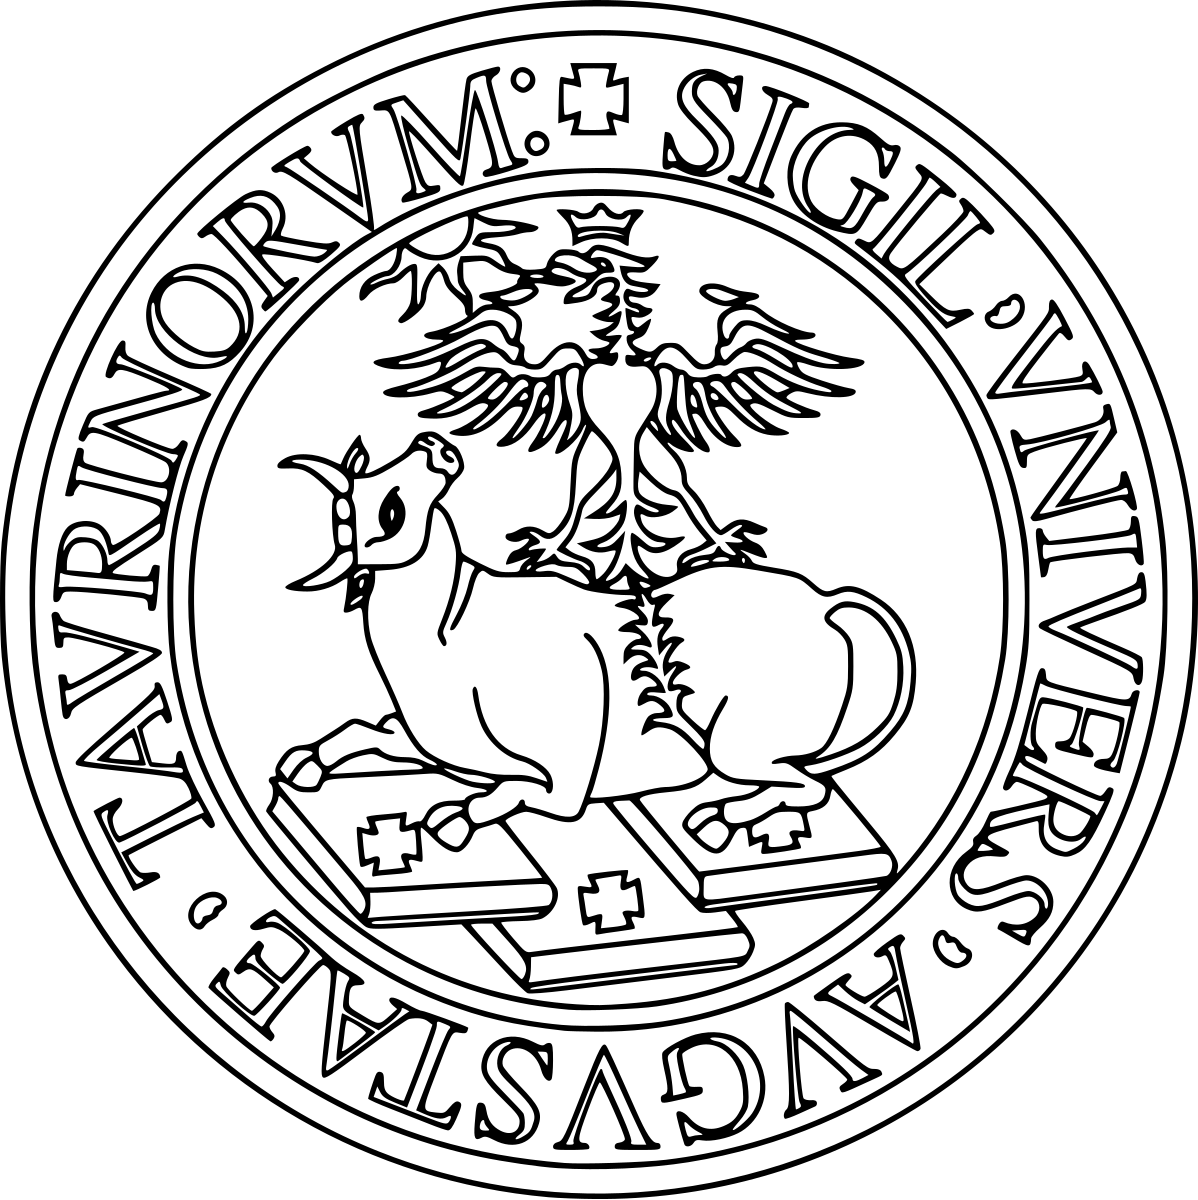
\includegraphics[width=4cm]{logo}}
%   \end{tabular}

\vskip 1.2cm

\centerline {\normalsize {Tesi di Laurea Triennale}} 

\vskip 0.7cm

\centerline{\Large {\bf Flusso di campi vettoriali su varietà e parentesi di Lie:}}
\centerline{\Large {\bf un approccio non standard.}}

\vskip 1.7cm

\noindent Relatore: Luca Motto Ros
\hfill  {Candidato: Davide Peccioli}



\vskip 2.7cm


\centerline{ANNO ACCADEMICO 2023-24}
\end{titlepage}
{\pagestyle{empty}
\null\cleardoublepage}


\fancyhead{} % cancella tutti i campi
\fancyfoot{}
\fancyhead[LE]{Flusso di campi vettoriali su varietà e parentesi di Lie: un approccio non standard.}
\fancyhead[RO]{Indice}
\fancyfoot[C]{\thepage}
\renewcommand{\headrulewidth}{0.4pt}
\renewcommand{\footrulewidth}{0pt}
\pagestyle{fancy}

\tableofcontents\cleardoublepage

\hdrnew{Flusso di campi vettoriali su varietà e parentesi di Lie: un approccio non standard.}

\mainmatter

\chapter*{Introduzione}

Questa tesi di Laurea triennale in Matematica si pone come obiettivo quello di dimostrare un ben noto risultato della geometria differenziale, ovvero il seguente teorema. 
\paragraph{Teorema} Se $ X $ e $ Y $ sono due campi vettoriali di classe $ C^{2} $ su una varietà differenziabile $ M $, i loro flussi commutano se e solo se $ [X,Y] \equiv 0 $.

L'approccio scelto utilizza strumenti dell'analisi non-standard. In particolare, nei capitoli 2 e 3 si fornisce una rigorosa trattazione della costruzione dell'estensione non-standard di $ \R $ ed una generalizzazione all'universo $ V(\R) $. Nel capitolo 4, infine, si utilizzano le basi teoriche poste in precedenza per definire l'estensione non standard di una varietà differenziabile $ M $, e per definire la naturale traduzione dei campi vettoriali in ambito infinitesimale. 

Con queste premesse, il flusso di un campo vettoriale, inizialmente definito come oggetto ``integrale'', diventa un cammino composto da passi infinitesimali. Questo consente una definizione formale di flusso che concordi con la intuizione naturale del concetto.
\chapter{Prerequisiti}\stepcounter{capitoloeccolo}

\section{Prerequisiti di Logica}

\lipsum[1]

\subsection{Assioma della scelta}

Per la costruzione di $ \starR $ come ultraprodotto, sarà necessario utilizzare l'Assioma della Scelta. Lo si presenta anche nella sua forma equivalente: il Lemma di Zorn

\paragrafo{Assioma di scelta}{%
    Per ogni insieme $ X\neq \emptyset $ esiste \[f:\parti{X}\setminus\{\emptyset\}\longrightarrow X\]tale che $ f(Y) \in Y $ per ogni $ Y \subseteq X $ non vuoto.
}{}{}
\paragrafo{Lemma di Zorn}{%
    Se un insieme (parzialmente) ordinato è tale che ogni catena ha un maggiorante, allora ha un elemento massimale.
}{}{}
\proposizione{odijcoijodijocijoijoijoi}{
    Sia $ F:\mathcal{N}\longrightarrow \mathcal{M} $ un'immersione. Le seguenti affermazioni sono equivalenti: \begin{enumerate}
        \item $ F $ è un'immersione elementare; 
        \item per ogni $ \mathcal{L} $-formula $ \varphi(y,x_1,\dots,x_{n} ) $ ed ogni $ a_1,\dots,a_{n} \in N  $ \[
            \mathcal{M}\vDash \exists y \, \varphi\left[y, F(a_1),\dots,F(a_{n}) \right]\qquad\text{sse}\qquad \parbox{15em}{$\mathcal{M}\vDash\varphi\left[F(a_{0}), F(a_1),\dots,F(a_{n}) \right]${ per qualche }$a_0 \in N.$}
        \]
    \end{enumerate}
}

\section{Prerequisiti di Geometria Differenziale}\label{sec:geodiff}

\lipsum[2]

\chapter{Campo dei reali non standard}\stepcounter{capitoloeccolo}

Si parla di modelli non standard dei numeri reali quando si considerano campi reali \emph{non archimedei}, che verifichino un certo principio di \straniero{transfer}: in questo modo le proprietà elementari dei numeri reali sono conservate. Inoltre, in questi campi, esistono numeri infinitesimi ed infiniti, che si comportano come utilizzati da Lebniz. 

In questo capitolo si costruirà formalmente un campo $ ^{*}\R $ di numeri reali non standard, e se ne vedranno le principali proprietà.

\definizione{
    Un campo ordinato $ \mathcal{K}=(\K, +,-, \cdot ,0,1,\le) $ si dice \emph{archimedeo} se per ogni $ x \in \K $, con $ 0<x $, esiste $ n \in \N $ tale che l'elemento \[\parentesi{n\text{-volte}}{1+\dots+1} \eqqcolon n1\]sia $ x<n1 $.
}

% % \section{Esistenza di un campo non archimedeo}

% \definizione{
%     Un campo ordinato $ \mathcal{K}=(\K, +,-, \cdot ,0,1,\le) $ si dice \emph{archimedeo} se per ogni $ x \in \K $, con $ 0<x $, esiste $ n \in \N $ tale che l'elemento \[\parentesi{n\text{-volte}}{1+\dots+1} \eqqcolon n1\]sia $ x<n1 $
% }
% \teorema{ijpijoijodijoijoijodijcoijoijoijoijoijoij}{
%     Per ogni campo ordinato archimedeo esiste un campo ordinato non archimedeo elementarmente equivalente al primo.    
% % Ogni campo ordinato è elementarmente equivalente ad un campo ordinato non Archimedeo. 
% }
% \dimostrazione{ijpijoijodijoijoijodijcoijoijoijoijoijoij}{
%     Si estenda il linguaggio dei campi: \[
%         \mathcal{L}_{\text{Fld}}=\{+,-, \cdot ,0,1,\le\} \subseteq \mathcal{L}'=\mathcal{L}_{\text{Fld}}\cup\{c\}
%     \]dove $ c $ è una costante, e si consideri una $\mathcal{L}_{\text{Fld}}$-struttura $ \mathcal{K}$. 

%     Sia ora $ T $ una $ \mathcal{L}'$-teoria:\[
%         T=\operatorname{Th}_{{\text{Fld}}}(\mathcal{K})\cup\{\tau_{n}: 1\le n \in \N \}
%     \]dove $ \tau_{n}  $ è l'enunciato $ n \cdot 1 \le c $.

%     $ T $ è finitamente soddisfacibile. Infatti, sia $ 1\le n \in \N $. Allora la $ \mathcal{L}' $-espasione $ \mathcal{K}_{n}  $ tale che $ c^{\mathcal{K}_{n} } = n \cdot 1 $ è tale che \[
%         \mathcal{K}_n \vDash \operatorname{Th}_{{\text{Fld}}}(\mathcal{K})\cup\{\tau_{i}: 1\le i \le n, i \in \N \}.
%     \]
    
%     Per il teorema di compattezza esiste $ \mathcal{F}' $, una $ \mathcal{L}' $-struttura tale che \[
%         \mathcal{F}'\vDash T'.
%     \]Se $ \mathcal{F} $ è la $ \mathcal{L}_{\text{Fld}} $-ridotta di $ \mathcal{F}' $, \[
%         \mathcal{F}=\left(A,+,-, \cdot ,0,1,\le\right)
%     \]allora in $ \mathcal{F} $ l'elemento $ c^{\mathcal{F}'} \in A $ è tale che $ n \cdot 1\le  c^{\mathcal{F}'} $ per ogni $ n\ge 1 $. 
    
%     $\implies$ $ \mathcal{F} $ non è Archimedeo e $ \mathcal{F} $ è elementarmente equivalente a $ \mathcal{K} $.\qed
% }

% \osservazione{
%     Il teorema \teoref{ijpijoijodijoijoijodijcoijoijoijoijoijoij} assicura che esista un campo $ \starR $ elementarmente equivalente ad $ \R $ ma non archimedeo. 
% }

\section{Costruzione degli iperreali}

L'obiettivo di questa sezione è costruire $ \starR $ come ultraprodotto di $ \mathcal{L}$-strutture.

\subsection{Prodotto di $ \mathcal{L} $-strutture}

\paragrafo{Prodotto Cartesiano}{%
    Sia $ (A_{i} )_{i \in I} $ una famiglia di insiemi non vuoti indicizzata su $ I\neq \emptyset $. Il \emph{prodotto cartesiano} degli $ A_{i}$ è l'insieme%
    \[
        \prod_{i \in I} A_{i}=\left\{f:I\longrightarrow \bigcup_{i \in I} A_{i}: f(i) \in A_{i}\text{ per ogni } i \in I  \right\}  
    \]Gli elementi $ f \in \prod_{i \in I} A_{i} $ si indicano come sequenze generalizzate $ \sequence{a_{i}}_{i \in I} $ dove $ a_{i}=f(i)  $ è la $ i $-esima coordinata di $ \sequence{a_{i} }_{i \in I} $ (o di $ f $) per ogni $ i \in I $. 

    Quando è chiaro l'insieme su cui varia $ i $, si userà $ \sequence{a_{i}} $ in luogo di $ \sequence{a_{i}}_{i \in I} $.

    Quando $ A_{i} =A $ per ogni $ i \in I $ si scriverà $ A^{I} $ invece di $ \prod_{i \in I} A_{i} $.
}{}{}
\paragrafo{Prodotto di strutture}{%
    Sia $ (\mathcal{A}_i)_{i \in I} $ una famiglia di $ \mathcal{L} $-strutture (con dominio, rispettivamente, $ A_{i}  $) indicizzata su $ I\neq \emptyset $. Il loro \emph{prodotto (diretto)} $ \prod_{i \in I} \mathcal{A}_{i} $ è la $ \mathcal{L} $-struttura $ \mathcal{M} $ con dominio $ \prod_{i \in I} A_{i} $ e simboli di $ \mathcal{L} $ interpretati come segue: \begin{itemize}
        \item per ogni $ R \in \operatorname{Rel} $ con arietà $ k $, ed ogni $ \sequence{a_{i}^{1}},\dots,\sequence{a_{i}^{k}} \in\prod_{i \in I} A_{i}$ \[
            \left(\sequence{a_{i}^{1}},\dots,\sequence{a_{i}^{k}}\right) \in R^{\mathcal{M}}\qquad \text{se e solo se}\qquad \left(a_{i}^{1}, \dots, a_{i}^{k}  \right) \in R^{\mathcal{A}_i}\text{ per ogni }i \in I;
        \]
        \item per ogni $ f \in \operatorname{Fun} $ con arietà $ k $, ed ogni $ \sequence{a_{i}^{1}},\dots,\sequence{a_{i}^{k}}, \sequence{b_{i} } \in\prod_{i \in I} A_{i}$ \[
            f^{\mathcal{M}}\left(\sequence{a_{i}^{1}},\dots,\sequence{a_{i}^{k}}\right) = \sequence{b_{i} }\qquad \text{se e solo se}\qquad \parbox{12em}{$f^{\mathcal{A}_i}\left(a_{i}^{1}, \dots, a_{i}^{k}  \right) = b_{i} $ per ogni $i \in I$;}
        \]
        \item per ogni $ c \in \operatorname{Cost} $ ed ogni $ \sequence{b_{i}} \in \prod_{i \in I}A_{i}   $ \[
            c^{\mathcal{M}}=\sequence{b_{i}}\qquad\text{se e solo se}\qquad c^{\mathcal{A}_i}=b_{i} \text{ per ogni }i \in I.
        \]
    \end{itemize}
}{}{}
\subsection{Filtri e ultrafiltri}

\definizione{
    Sia $ I\neq \emptyset $ un insieme. Una famiglia non vuota $ \mathcal{F} \subseteq \parti{I} $ è un \emph{filtro} se soddisfa le seguenti proprietà;\begin{itemize}
        \item se $ A \in \mathcal{F} $ e $ A \subseteq B \subseteq I $, allora $ B \in \mathcal{F} $;
        \item se $ A,B \in \mathcal{F} $, allora $ A \cap B \in \mathcal{F}$.
    \end{itemize}

    Un filtro $ \mathcal{F} $ si dice \emph{proprio} se $ \emptyset\notin \mathcal{F} $.
}
\definizione{
    Il \emph{filtro di Fréchet} $ \mathcal{F}_{\text{Fr}}^{I} $ su $ I $ è definito nel seguente modo:\citazione{$ A \in \mathcal{F}_{\text{Fr}}^{I} $ se e solo se $ I\setminus A $ è finito.}
}
\paragrafo{FIP}{%
    Una famiglia $ \mathcal{G} \subseteq\parti{I} \setminus\{\emptyset\}$ ha la \emph{proprietà dell'intersezione finita} (brevemente FIP) se ogni intersezione finita di elementi di $ \mathcal{G} $ è non vuota.
}{}{}
\paragrafo{Estensione canonica}{%
    Ogni famiglia $ \mathcal{G}\subseteq\parti{I} \setminus\{\emptyset\}$ con la FIP si estende canonicamente al filtro proprio\[
        \langle \mathcal{G}\rangle =\{ B \subseteq I: B \supseteq A_1\cap\dots\cap A_{k}\text{ per qualche }k \in \N\text{ e }A_1,\dots,A_{k} \in \mathcal{G}\}.
    \]Equivalentemente, $ \langle \mathcal{G}\rangle $ è il più piccolo filtro su $ I $ che contiene $ G $
}{}{}
\paragrafo{Osservazione}{%
    $ \langle \mathcal{G}\rangle $ è un filtro proprio. Infatti:\begin{itemize}
        \item se $ A \in \langle \mathcal{G}\rangle $, allora per qualche $ A_1,\dots,A_{k} \in \mathcal{G}  $ \[
            A \supseteq A_1 \cap \dots\cap A_{k} 
        \]e se $ B \supseteq A $ allora \[
            B \supseteq A_1 \cap \dots\cap A_{k} 
        \]e quindi $ B \in \langle \mathcal{G}\rangle $; 
        \item se $ B_1, B_2 \in \langle \mathcal{G}\rangle $, allora \begin{align*}
            B_1 &\supseteq A_1\cap \dots\cap A_{k}\\
            B_2 &\supseteq C_1\cap \dots\cap C_{k}
        \end{align*}e allora \[
            B_1\cap B_2 \supseteq A_1\cap \dots\cap A_{k}\cap C_1\cap \dots\cap C_{k}
        \]e quindi $ B_1\cap B_2 \in \langle \mathcal{G}\rangle$. 
    \end{itemize}

    La condizione FIP di $ \mathcal{G} $ garantisce che $ \langle \mathcal{G}\rangle $ sia un filtro \emph{proprio}, ma è possibile costruire un filtro in questo modo a partire da una qualsiasi famiglia di sottoinsiemi di $ I $. 
}{}{}
\definizione{
    Un filtro proprio $ \mathcal{F} $ su $ I $ si dice \begin{itemize}
        \item \emph{ultrafiltro} se per ogni $ A \subseteq I $ si ha $ A \in \mathcal{F} $ o $ I\setminus A \in \mathcal{F} $; 
        \item \emph{primo} se $ A\cup B \in \mathcal{F} $ implica che $ A \in \mathcal{F} $ o $ B \in \mathcal{F} $;
        \item \emph{massimale} se non esiste un filtro proprio $ \mathcal{F}' $ su $ I $ tale che $ \mathcal{F}' \supsetneqq \mathcal{F} $.
    \end{itemize}
}
\proposizione{doijcoijoosijoijoijdcidicoijcoijdoijoijoij}{
    Dato $ I \neq \emptyset$, $ \mathcal{F} $ filtro proprio su $ I $, allora sono fatti equivalenti: \begin{enumerate}
        \item $ \mathcal{F} $ è un ultrafiltro;
        \item $ \mathcal{F} $ è primo;
        \item $ \mathcal{F} $ è massimale.
    \end{enumerate} 
}
\dimostrazioneprop{doijcoijoosijoijoijdcidicoijcoijdoijoijoij}{
    $ \boxed{1.\Rightarrow 2.} $\hspace{1em} Per assurdo, $ A\cup B \in \mathcal{F} $, ma $ A, B\notin \mathcal{F} $. 
    
    Per $ 1. $ si ha che $ I \setminus A, I \setminus B \in \mathcal{F} $. Allora\[
        \parentesi{=I\setminus (A\cup B)}{(I\setminus A) \cap (I \setminus B)} \in \mathcal{F}
    \]che è un assurdo perché $ \mathcal{F} $ è proprio.

    $ \boxed{2.\Rightarrow 3.} $\hspace{1em} Si supponga per assurdo che esista un filtro proprio $ \mathcal{F}'\supsetneqq \mathcal{F} $. Sia $ A \in \mathcal{F}' \setminus \mathcal{F} $. 
    
    In particolare, $ I \setminus A \notin \mathcal{F}' $, quindi $ I \setminus A \notin \mathcal{F}$. 
    
    Ma $ A \cup (I\setminus A) = I \in \mathcal{F} $, e $ A, I\setminus A \notin \mathcal{F} $, il che contraddice 2.

    $ \boxed{3.\Rightarrow 1.} $\hspace{1em} Si supponga per assurdo che $ A \notin \mathcal{F} $ e $ I\setminus A \notin \mathcal{F} $. 
    
    Sia $ \mathcal{G}=\mathcal{F}\cup \{A\} $. $ \mathcal{G} $ ha la FIP\footnote{Infatti, siano $ A_1,\dots,A_{k} \in \mathcal{G}   $, senza perdita di generalità assunti tutti diversi. Se $ A_1,\dots,A_{k} \in \mathcal{F}  $, allora $ A_1\cap\dots\cap A_{k}\neq \emptyset  $ perché $ \mathcal{F} $ è un filtro proprio. Se invece $ A_{k} = A  $, allora \[
        \parentesi{ \in \mathcal{F}}{A_1\cap \dots\cap A_{k-1} }\cap A =  B \cap A
    \]con $B = A_1\cap \dots\cap A_{k-1}$. Se capitasse che $ B\cap A =\emptyset$, allora $ B \subseteq I\setminus A $, da cui $ I\setminus A \in \mathcal{F} $, assurdo poiché per ipotesi $ I \setminus A \notin \mathcal{F} $.}. Sia ora $ \mathcal{F}'=\langle \mathcal{G}\rangle $. $ \mathcal{F}' $ è un filtro proprio, e si ha \[
        \mathcal{F}' \supseteq \mathcal{G}\supseteq \mathcal{F}, \qquad \mathcal{F}'\neq \mathcal{F}
    \]poiché $ A \in \mathcal{F}'\setminus \mathcal{F} $. Questo contraddice 3.\qed
}
\definizione{
    Un ultrafiltro $ \mathcal{U} $ su $ I $ si dice \emph{non principale} se per ogni $ A \subseteq I $ finito, $ I\setminus A \in \mathcal{U} $.
}
\paragrafo{Lemma degli ultrafiltri}{%
    Ogni filtro proprio $ \mathcal{F} $ su $ I $ può essere esteso ad un ultrafiltro $ \mathcal{U}\supseteq \mathcal{F} $ su $ I $.
}{doijcsoijoijoijoijoijoijoij}{}
\dimostrazioneprop{doijcsoijoijoijoijoijoijoij}{
    Sia $ X=\{\mathcal{G}: \mathcal{G} \supseteq \mathcal{F}, \mathcal{G}\text{ filtro proprio su }I\} $. 

    Si consideri $ (X, \subseteq)$: sia $ C \subseteq X $ una catena, cioè se $ \mathcal{G}, \mathcal{G}' \subseteq C $ allora o $ \mathcal{G} \subseteq \mathcal{G}' $ oppure $ \mathcal{G}' \subseteq \mathcal{G} $. 

    Sia $ \displaystyle \mathcal{H} = \bigcup_{\mathcal{G} \in C} \mathcal{G} $. 
    
    È evidente che per ogni $ \mathcal{G} \in C $, $ \mathcal{G} \subseteq \mathcal{H} $. Necessariamente $\emptyset \notin \mathcal{H}$ perché $ \mathcal{H} $ unione di filtri propri, e inoltre $ \mathcal{H} \supseteq \mathcal{F} $ poiché unione di filtri che contengono $ \mathcal{F} $. Inoltre $ \mathcal{H} $ è un filtro. Infatti: \begin{itemize}
        \item \emph{chiusura per sovrainsiemi}: se $ A \in \mathcal{H} $, allora $ A \in \mathcal{G} $ per qualche $ \mathcal{G} \in C $ dunque, per ogni $ B \supseteq A $ necessariamente $ B \in \mathcal{G} $, poiché $ \mathcal{G} $ è filtro, e dunque $ B \in \mathcal{H} $;
        \item \emph{intersezioni finite}: siano $ A, B \in \mathcal{H} $: si ha che $ A \in \mathcal{G} $ e $ B \in \mathcal{G}' $, per qualche $ \mathcal{G}, \mathcal{G}'  \in C$; poiché $ C $ è una catena, allora necessariamente deve valere una delle seguenti: \[
            A, B \in \mathcal{G} \supseteq \mathcal{G}',\qquad A, B \in \mathcal{G}' \supseteq \mathcal{G};
        \]e quindi $ A\cap B \in \mathcal{G} $ (oppure $ A\cap B \in \mathcal{G}' $) poiché $ \mathcal{G} $ (oppure $ \mathcal{G}' $) è un filtro. Dunque $ A\cap B \in \mathcal{H} $.
    \end{itemize}

    Per il lemma di Zorn, esiste $ \mathcal{U} $ massimale in $ X $, e necessariamente $ \mathcal{U} \supseteq \mathcal{F} $. Dunque $ \mathcal{U} $ è un filtro massimale rispetto alla famiglia di tutti i filtri su $ I $\footnote{Se per assurdo $ \mathcal{U} $ non fosse un ultrafiltro massimale, sia $ \mathcal{U}' \supsetneqq \mathcal{U} $ un filtro proprio su $ I $. Dunque $ \mathcal{U}' \supseteq \mathcal{F}$ e $ \mathcal{U}' $ filtro proprio su $ I $, e quindi $ \mathcal{U}' \in X $. Questo contraddice il risultato secondo cui $ \mathcal{U} $ è massimale in $ X $.}, e per la proposizione \framref{doijcoijoosijoijoijdcidicoijcoijdoijoijoij}, un filtro massimale è un ultrafiltro.\qed
}
\subsection{Ultraprodotto di $ \mathcal{L} $-strutture}

\definizione{
    Sia $ (A_{i} )_{i \in I} $ una famiglia di insiemi non vuota indicizzata da $ I \neq \emptyset $. Dato un filtro $ \mathcal{F} $ su $ I $ si definisce la relazione di equivalenza $ \sim_{\mathcal{F}}  $ su $ \prod_{i \in I} A_{i}   $ ponendo per $ \sequence{a_i},\sequence{b_i} \in \prod_{i \in I} A_{i} $ \[
        \sequence{a_i}\sim_{\mathcal{F}}\sequence{b_i}\qquad\text{se e solo se}\qquad \{i \in I:a_i=b_i \} \in \mathcal{F}. 
    \]La classe di equivalenza rispetto a $ \sim_{\mathcal{F}}$ di un elemento $ \sequence{a_i} \in \prod_{i \in I}A_{i}$ verrà indicata con $ [\sequence{a_i}] $
}
\osservazione{
    $ \sim_{\mathcal{F}} 
    $ è una relazione di equivalenza: simmetria e riflessività sono ovvie; per la transitività: siano $ \sequence{a_i}\sim_{\mathcal{F}} \sequence{b_i} $, e $ \sequence{b_i}\sim_{\mathcal{F}}\sequence{c_i} $. Allora \begin{align*}
            X_{\sequence{a_i},\sequence{b_i}}&\coloneqq\{i \in I: a_i = b_i\} \in \mathcal{F}\\
            X_{\sequence{b_i},\sequence{c_i}}&\coloneqq\{i \in I: b_i = c_i\} \in \mathcal{F}
        \end{align*}

    Si deve dimostrare che l'insieme $ X_{\sequence{a_i},\sequence{c_i}} \coloneqq\{i \in I: a_i = b_i\} \in \mathcal{F}$, ma \[
        X_{\sequence{a_i},\sequence{b_i}} \cap X_{\sequence{b_i},\sequence{c_i}} \subseteq X_{\sequence{a_i},\sequence{c_i}}   
    \]ma $ X_{\sequence{a_i},\sequence{b_i}} \cap X_{\sequence{b_i},\sequence{c_i}} \in \mathcal{F} $, e dunque $ X_{\sequence{a_i},\sequence{c_i}} \in \mathcal{F} $.
}
\paragrafo{Prodotto ridotto di insiemi}{%
    Il \emph{prodotto ridotto} $ \prod_{{\mathcal{F}}} A_{i}$ degli $ A_{i}  $ modulo $ \mathcal{F} $ è il quoziente \[
        \prod_{i \in I}A_{i}/\sim_{\mathcal{F}} = \left\{\left[\sequence{a_{i}}\right]: \sequence{a_{i}} \in \prod_{i \in I}A_{i}  \right\}. 
    \]Se $ \mathcal{F} $ è un ultrafiltro, il prodotto ridotto corrispondente $ \prod_{\mathcal{F}}A_{i}   $ si dice \emph{ultraprodotto}. Quando $ A_{i}=A  $ per ogni $ i \in I $, si parla invece di \emph{potenza ridotta} e scriviamo $ A^{I}/\mathcal{F} $; se $ \mathcal{F} $ è un ultrafiltro, si parla di \emph{ultrapotenza}.
}{}{}
\paragrafo{Ultraprodotto di strutture}{%
    Sia $ (\mathcal{A}_i)_{i \in I} $ una famiglia di $ \mathcal{L} $-strutture indicizzata da $ I\neq \emptyset $, e sia $ \mathcal{U} $ un ultrafiltro su $ I $. L'ultraprodotto $ \prod_{\mathcal{U}}\mathcal{A}_i  $ è la $ \mathcal{L} $-struttura $ \mathcal{M} $ con dominio $ \prod_{\mathcal{U}}A_{i}   $ e simboli di $ \mathcal{L} $ interpretati come segue: \begin{itemize}
        \item per ogni $ R \in \operatorname{Rel} $ con arietà $ k $ ed ogni $ \sequence{a_{i}^{1}},\dots,\sequence{a_{i}^{k}} \in \prod_{i \in I}A_{i}  $%
            \begin{gather*}
                \left(\left[\sequence{a_{i}^{1}}\right],\dots,\left[\sequence{a_{i}^{k}}\right]\right) \in R^{\mathcal{M}}\\ 
                \text{se e solo se}\\ 
                \left\{i \in I: \left(a_{i}^{1}, \dots, a_{i}^{k}  \right) \in R^{\mathcal{A}_i}\right\} \in \mathcal{U};
            \end{gather*}
        \item per ogni $ f \in \operatorname{Fun} $ con arietà $ k $ ed ogni $ \sequence{a_{i}^{1}},\dots,\sequence{a_{i}^{k}} ,\sequence{b_{i} } \in \prod_{i \in I}A_{i}  $%
            \begin{gather*}
                f^{\mathcal{M}}\left(\left[\sequence{a_{i}^{1}}\right],\dots,\left[\sequence{a_{i}^{k}}\right]\right)=\left[\sequence{b_{i} }\right]\\ 
                \text{se e solo se}\\ 
                \left\{i \in I: f^{\mathcal{A}_i}\left(a_{i}^{1}, \dots, a_{i}^{k}  \right) = b_{i} \right\} \in \mathcal{U};
            \end{gather*}
        \item per ogni $ c \in \operatorname{Cost} $ ed ogni $ \sequence{b_{i} } \in \prod_{i \in I}A_{i}   $ \[
            c^{\mathcal{M}}=\left[\sequence{b_{i} }\right]\qquad\text{se e solo se}\qquad \{i \in I: c^{\mathcal{A}_i}=b_{i} \} \in \mathcal{U}.
        \]
    \end{itemize}
    Se $ \mathcal{A}_i = \mathcal{A}$ per ogni $  i \in I $, la $ \mathcal{L} $-struttura $ \mathcal{A}^{I}/\mathcal{U} $ si dice \emph{ultrapotenza} di $ \mathcal{A} $.
}{dcjkklkmdjjjjultraprodottoinssimo}{}
\osservazione{
    Le definizioni sopra riportate sono ben date. A titolo esplicativo si dimostra che se $ R $ è un simbolo di relazione binario, e $ \sequence{a^{1}_i}, \sequence{a^{2}_i },\sequence{b^{1}_i}, \sequence{b^{2}_i } \in \prod_{i \in I} A_{i}  $ con \begin{equation*}
        \sequence{a_{i}^{1} } \sim_{\mathcal{U}} \sequence{b_{i}^{1} } ,\qquad \sequence{a_{i}^{2} } \sim_{\mathcal{U}} \sequence{b_{i}^{2} } 
    \end{equation*}allora $  \left\{i \in I: \left(a_{i}^{1}, a_{i}^{2}  \right) \in R^{\mathcal{A}_i}\right\} \in \mathcal{U} $ se e solo se $  \left\{i \in I: \left(b_{i}^{1}, b_{i}^{2}  \right) \in R^{\mathcal{A}_i}\right\} \in \mathcal{U} $. Per simmetria si dimostra un'unica implicazione.

    Per definizione, i seguenti insiemi appartengono ad $ \mathcal{U} $: \begin{equation*}
        \set{i \in I: a^{1}_i = b^{1}_i}, \quad\set{i \in I: a^{2}_i = b^{2}_i}. 
    \end{equation*}Inoltre vale \begin{equation*}
        \set{i \in I: \left(a_{i}^{1}, a_{i}^{2}  \right) \in R^{\mathcal{A}_i}}\cap\set{i \in I: a^{1}_i = b^{1}_i}\cap\set{i \in I: a^{2}_i = b^{2}_i} \subseteq \set{i \in I: \left(b_{i}^{1}, b_{i}^{2}  \right) \in R^{\mathcal{A}_i}}
    \end{equation*}infatti, fissato $ i \in I $, se $ \left(a_{i}^{1}, a_{i}^{2}  \right) \in R^{\mathcal{A}_i} $ e $ a_{i}^{1} = b_{i}^{1}   $ e $ a_{i}^{2} = b^{2}_i  $, allora $ \left(b_{i}^{1},b_{i}^{2}  \right) = \left(a_{i}^{1}, a_{i}^{2}  \right) \in R^{\mathcal{A}_i}$.

    Questo dimostra la buona definizione della definizione precedente nel caso in una relazione binaria.
}
\proposizione{doijcoijdijcijijoijoijoijcoaijoijoijoij}{
    Sia $ (\mathcal{A}_i)_{i \in I} $ una famiglia di $ \mathcal{L} $-strutture (con dominio, rispettivamente, $ A_{i}  $) indicizzata su $ I \neq \emptyset $, e sia $ \mathcal{U} $ un ultrafiltro su $ I $. Per ogni $ \mathcal{L} $-termine $ t(x_1,\dots,x_{n} ) $ ed ogni $ \sequence{a_{i}^{1}},\dots,\sequence{a_{i}^{n}} ,\sequence{b_{i} } \in \prod_{i \in I}A_{i}   $\begin{gather*}
        t^{\mathcal{M}}\left(\left[\sequence{a_{i}^{1}}\right],\dots,\left[\sequence{a_{i}^{k}}\right]\right)=\left[\sequence{b_{i} }\right]\\ 
        \text{se e solo se}\\ 
        \left\{i \in I: t^{\mathcal{A}_i}\left(a_{i}^{1}, \dots, a_{i}^{k}  \right) = b_{i} \right\} \in \mathcal{U};
    \end{gather*}
}
\dimframmento{doijcoijdijcijijoijoijoijcoaijoijoijoij}{
    Si dimostra per induzione sulla complessità del termine. \begin{itemize}
        \item \emph{Caso base:} i termini di complessità minima sono le costanti e le variabili. Nel caso in cui il termine $ t $ sia una costante, il risultato è valido per definizione di ultraprodotto. 
        
        Quanto $ t(x): x $ è una costante, fissati $ \sequence{a_{i} },\sequence{b_{i} } \in \prod_{i \in I} A_{i}   $, \begin{equation*}
            t^{\mathcal{M}}\left(\left[\sequence{a_{i} }\right]\right) = \left[\sequence{b_{i} }\right]
        \end{equation*}se e solo se $ \left[\sequence{a_{i} }\right]=\left[\sequence{b_{i} }\right] $, ovvero, per definizione di classi di equivalenze, se e solo se \begin{equation*}
            \set{i \in I: t^{\mathcal{A}_i}(a_{i} ) = b_{i} }=\set{i \in I: a_{i} = b_{i}  } \in \mathcal{U}.
        \end{equation*}
        \item \emph{Passo induttivo:} siano $ t_1(x_1,\dots,x_{n} ), \dots, t_k(x_1,\dots,x_{n} ) $ termini per cui valga il risultato, e sia $ f $ simbolo di funzione di arietà $ k $. 
        
        Sia dunque $ t(x_1,\dots,x_{n}) $ il termine \begin{equation*}
            f\left(t_1(x_1,\dots,x_{n} ), \dots, t_{k}(x_1,\dots,x_{n} ) \right).
        \end{equation*} \commento{Non sono riuscito a terminare questa dimostrazione}
        % Fissati $ \sequence{a^{1}_i},\dots,\sequence{a^{n}_i}, \sequence{b_{i} } \in \prod_{i \in I} A_{i}  $, si dimostrerà che \begin{equation*}
        %     t^{\mathcal{M}}\left(\left[\sequence{a^{1}_i}\right],\dots,\left[\sequence{a^{n}_i}\right]\right) = \left[\sequence{t^{\mathcal{A}_i}\left(a^{1}_i,\dots,a^{n}_i\right)}\right].
        % \end{equation*}Questo corrisponde alla tesi.
        % % \begin{equation*}
        % %     t_{j}^{\mathcal{M}}\left(\left[\sequence{a^{1}_i}\right],\dots,\left[\sequence{a^{n}_i}\right]\right) = \left[\sequence{c^{j}_i}\right]
        % % \end{equation*}per qualche $ \sequence{c^{j}_i} \in \prod_{i \in I} A_{i}   $.

        % Dunque $ t^{\mathcal{M}} \left(\left[\sequence{a^{1}_i}\right],\dots,\left[\sequence{a^{n}_i}\right]\right) = \left[\sequence{b_i}\right]$ se e solo se \begin{equation*}
        %     f^{\mathcal{M}}\left(t_{1}^{\mathcal{M}}\left(\left[\sequence{a^{1}_i}\right],\dots,\left[\sequence{a^{n}_i}\right]\right),\dots,t_{k}^{\mathcal{M}}\left(\left[\sequence{a^{1}_i}\right],\dots,\left[\sequence{a^{n}_i}\right]\right)\right) = \left[\sequence{b_{i} }\right]
        % \end{equation*}e a sua volta questo è equivalente ad \begin{equation}
        %     f^{\mathcal{M}}\left(\left[\sequence{c^{1}_i}\right],\dots,\left[\sequence{c^{k}_i}\right]\right) = \left[\sequence{b_{i} }\right].\label{eq:ciaonen}
        % \end{equation}Per la definizione di funzioni in un ultraprodotto, \eqref{eq:ciaonen} se e solo se \begin{equation*}
        %     B \coloneqq \set{i \in I: f^{\mathcal{A}_i}\left(c^{1}_i,\dots,c^{k}_i\right)=b_{i} } \in \mathcal{U}.
        % \end{equation*}Si considerino ora gli insiemi \begin{align*}
        %     B' &\coloneqq\set{i \in I: t^{\mathcal{A}_i}(a^{1}_i,\dots,a^{n}_i) = b_{i} },\\ 
        %     B''&\coloneqq B\cap \set{i \in I: t_{1}^{\mathcal{A}_i}(a^{1}_i,\dots,a^{n}_i) = c^{1}_i }\cap \dots \cap \set{i \in I: t_{k}^{\mathcal{A}_i}(a^{1}_i,\dots,a^{n}_i) = c^{k}_i }
        % \end{align*}L'inclusione $ B'' \subseteq B' $ è banale, e pertanto se $ B \in \mathcal{U} $ allora $ B' \in \mathcal{U}$, poiché $ \mathcal{U} $ è un filtro.

        % Viceversa, se $ B' \in \mathcal{U}$,
    \end{itemize}
}
\teorema[Teorema di Łoś]{dsoijsocijoijdididcoijdoijoijoicjoijoijocijoijoijcoijoijoij}{
    Sia $ (\mathcal{A}_i)_{i \in I} $ una famiglia di $ \mathcal{L} $-strutture (con dominio, rispettivamente, $ A_{i}  $) indicizzata su $ I \neq \emptyset $, e sia $ \mathcal{U} $ un ultrafiltro su $ I $. Sia $ \mathcal{M}\coloneqq\prod_{\mathcal{U}} \mathcal{A}_{i}   $. Per ogni $ \mathcal{L} $-formula $ \varphi(x_1,\dots,x_{n} ) $ e per ogni $\sequence{a_{i}^{1}},\dots,\sequence{a_{i}^{n}} \in\prod_{i \in I} A_{i}$, si ha \[
        \mathcal{M}\vDash \varphi\left[\left[\sequence{a_{i}^{1} }\right],\dots,\left[\sequence{a_{i}^{n} }\right]\right]\quad\text{se e solo se}\quad X_{\varphi, \sequence{a_{i}^{1}},\dots,\sequence{a_{i}^{n}}} \in \mathcal{U}
    \]dove $ X_{\varphi, \sequence{a_{i}^{1}},\dots,\sequence{a_{i}^{n}}} = \left\{i \in I: A_{i}\vDash \varphi\left[a_{i}^{1},\dots,a_{i}^{n}  \right] \right\} $
}
\dimostrazione{dsoijsocijoijdididcoijdoijoijoicjoijoijocijoijoijcoijoijoij}{
    Si dimostra il teorema per induzione sull'altezza della formula. \begin{itemize}
        \item \emph{Caso base:} per dimostrare il caso di una $ \mathcal{L}$-formula atomica, per semplicità, si considererà un simbolo di relazione binaria $ R $ e la formula $ \varphi: R(t_1,t_2) $. 
        
        Siano dunque $ \left[\sequence{b^{1}_i}\right] = t_1^{\mathcal{M}},\quad \left[\sequence{b^{2}_i}\right] = t_2^{\mathcal{M}} $. Necessariamente, per definizione di termine in un ultraprodotto, \begin{align*}
            X_{t_1}&=\{i \in I: t_1^{\mathcal{A}_i} = b_{i}^{1} \} \in \mathcal{U},\\
            X_{t_2}&=\{i \in I: t_2^{\mathcal{A}_i} = b^{2}_i\} \in \mathcal{U}.
        \end{align*}
        
        Per definizione, $ \mathcal{M}\vDash R(t_1,t_2) $ se e solo se $ \left[\sequence{b^{1}_i}\right] R^{\mathcal{M}} \left[\sequence{b^{2}_i}\right] $ e, per la definizione di relazione in un ultraprodotto, questo si verifica se e solo se $ X_{R} \in \mathcal{U}  $, dove \[
            X_{R}=\{i \in I: b^{1}_i\, R^{\mathcal{\mathcal{A}}_i}\, b^{2}_i\}.
        \]

        % Si ha che $ X_{R} \in \mathcal{U}  $ sse 
        Sia ora\[
            X=\{i \in I: b^{1}_i\, R^{\mathcal{\mathcal{A}}_i}\, b^{2}_i\,\text{ e }\,t_1^{\mathcal{A}_i} = b_{i}^{1}\,\text{ e }\,t_2^{\mathcal{A}_i} = b^{2}_i\}.
        \]$X \in \mathcal{U}$ se e solo se $ X_{R} \in \mathcal{U} $, poiché $ X_{R}\cap X_{t_1} \cap X_{t_2} \subseteq X$ e $ \mathcal{U} $ è un ultrafiltro.

        Ma $ \displaystyle X = \{i \in I: \mathcal{A}_i\vDash R(t_1,t_2)\} = X_{\varphi} $, e si è quindi dimostrata la tesi.
        \item \emph{Ipotesi induttiva:} l'ipotesi induttiva si verifica unicamente per i connettori e quantificatori logici $ \lnot, \lor, \exists$, in quanto tutti i rimanenti sono esprimibili come combinazione di questi.
        \begin{itemize}
            \item \emph{Negazione:} sia $ \varphi $ la formula $ \lnot\,\psi $, tale che il teorema valga per $ \psi $. 
            
            Per definizione $ \mathcal{M}\vDash \varphi $ se e solo se $ \mathcal{M}\nvDash \psi $, e, per ipotesi induttiva, questo è valido se e solo se $ \quad X_{\psi}\notin \mathcal{U}  $.
            
            Ma $ X_{\psi}\notin\mathcal{U}  $ se e solo se $ X_{\varphi} \in \mathcal{U}  $, poiché $ X_{\varphi}=I\setminus X_{\psi} $ e $ \mathcal{U} $ è ultrafiltro.
            \item \emph{Disgiunzione:} sia $ \varphi $ la formula $ \psi \,\lor\, \chi $, tale per cui il teorema valga per $ \psi $ e $ \chi $. 
            
            Per definizione $ \mathcal{M}\vDash \varphi $ se e solo se $ \mathcal{M}\vDash \psi $ oppure $ \mathcal{M}\vDash \chi $, e, per ipotesi induttiva, questo è equivalente a 
            \[
                X_{\psi} \in \mathcal{U}\,\text{ o }\,X_{\chi} \in \mathcal{U}  
            \]Inoltre, poiché $ \mathcal{U} $ è un filtro primo (condizione equivalente ad essere ultrafiltro) \[
                X_{\psi} \in U\,\text{ o }\,X_{\chi} \in \mathcal{U} \quad\text{se e solo se}\quad X_{\psi}\cup X_{\chi} \in \mathcal{U}   
            \]e, visto che $ X_{\varphi} = X_{\psi \,\lor\,\chi} = X_{\psi}\cup X_{\chi}     $, questo dimostra la tesi.
            \item \emph{Esistenziale:} sia $ \varphi $ la formula $ \exists y \, \psi(y) $, tale per cui il teorema valga per $ \psi(y) $. 
            
            $ \mathcal{M}\vDash \exists y \, \psi(y)$ se e solo se esiste $ \sequence{b_{i} } \in \prod_{i \in I} A_{i} $ tale per cui $ \mathcal{M}\vDash \psi\left[\left[\sequence{b_{i} }\right]\right] $. 
            
            Se esiste $\sequence{b_{i} } \in \prod_{i \in I} A_{i} $ tale per cui $ \mathcal{M}\vDash \psi\left[\left[\sequence{b_{i} }\right]\right]$, allora $ X_{\psi, \sequence{b_{i}}} \in \mathcal{U} $ per ipotesi induttiva. Inoltre, $ X_{\psi, \sequence{b_{i} }} \subseteq X_{\varphi} $ poiché \begin{align*}
                X_{\psi,\sequence{b_i}} &= \{ i \in I: \mathcal{A}_i\vDash \psi\left[b_{i} \right]\}\\ 
                X_{\varphi} &= \{i \in I: \mathcal{A}_i\vDash \exists\, y\,\psi\} 
            \end{align*}e quindi $ X_{\varphi} \in \mathcal{U}$ poiché $ \mathcal{U} $ è un ultrafiltro.
            
            Viceversa, se $ X_{\varphi} \in \mathcal{U}$, per ogni $ i \in  X_{\varphi}  $ sia un $ a_{i} \in A_{i}$ fissato tale che $ \mathcal{A}_i \vDash \psi[a_{i} ]$ (utilizzando l'assioma di scelta). Per ogni $ i \notin X_{\varphi}  $, sia $ c_{i} \in A_{i}$ scelto in maniera arbitraria. 

            Si definisce ora $ \sequence{b_{i} } \in \prod_{i \in I}A_{i}$: \[
                b_{i}  = \begin{cases}
                    a_{i} & i \in X_{\varphi}\\ 
                    c_{i} & i \notin X_{\varphi}     
                \end{cases} 
            \]e si ha che, necessariamente, \[
                X_{\psi,\sequence{b_{i}}} = \left\{i \in I: \mathcal{A}_i\vDash \psi\left[b_{i} \right]\right\} \supseteq X_{\varphi} \in \mathcal{U}
            \]e dunque $ X_{\psi,\sequence{b_{i}}} \in \mathcal{U}  $. Per ipotesi induttiva, $ \mathcal{M}\vDash\psi\left[\left[\sequence{b_{i} }\right]\right] $, e quindi $ \mathcal{M}\vDash \exists y\,\psi(y) $.\qed
        \end{itemize}
    \end{itemize}
}
\paragrafo{Corollario}{%
    Sia $ \mathcal{A} $ una $ \mathcal{L} $-struttura e $ \mathcal{U} $ un ultrafiltro su $ I $. Sia $ \pi: \mathcal{A}\longrightarrow \mathcal{A}^{I}/\mathcal{U} $ definita da $ \pi(a)=[\sequence{a_{i} }] $ dove $ a_{i} \equiv a $ per ogni $ i \in I $. Allora $ \pi $ è un'immersione elementare e, in particolare, $ \mathcal{A} $ e $ \mathcal{A}^{I}/\mathcal{U} $ sono elementarmente equivalenti.
}{dkjnckjjjjjjjjjjjjjdjjjjjdjnkjnkjn}{}
\dimframmento{dkjnckjjjjjjjjjjjjjdjjjjjdjnkjnkjn}{
    $ \pi $ è un morfismo. Questo segue banalmente dalla definizione degli elementi di $ \mathcal{A}^{I}/\mathcal{U} $, tenendo in considerazione che $ I \in \mathcal{U} $. 

    Si indichi con $ A $ il dominio di $ \mathcal{A} $, e con $ A^{I}/\mathcal{U} $ il dominio di $ \mathcal{A}^{I}/\mathcal{U} $.

    Per dimostrare che $ \pi $ sia una immersione elementare si sfrutta la proposizione \framref{odijcoijodijocijoijoijoi}. Si vuole dimostrare che per ogni $ \mathcal{L} $-formula $ \phi(y,x_1,\dots,x_{n}) $ e per ogni $ a^{1},\dots,a^{n} \in A $, \begin{gather}
        \mathcal{A}^{I}/\mathcal{U}\vDash \exists y \,\phi\left[y,\pi(a^{1}), \dots, \pi(a^{n})\right]\label{eq:uno}\\ 
        \text{se e solo se}\notag\\ 
        \mathcal{A}^{I}/\mathcal{U}\vDash \phi\left[\pi(a^{0}),\pi(a^{1}), \dots, \pi(a^{n})\right]\label{eq:due}
    \end{gather}per qualche $ a^{0} \in A $.

    Per il teorema di Łoś, ricordando che $ \pi(a^{k}) = [\sequence{a^{k}_i}] $ in cui $ a^{k}_i \equiv a^{k}$ per ogni $ i \in I $, \eqref{eq:uno} è verificata se e solo se \begin{equation*}
        X'  =\set{i \in I: \mathcal{A}\vDash \exists y\,\phi\left[y,a^{1}_i, \dots, a^{n}_i\right]}  \in \mathcal{U}
    \end{equation*}Dal momento che $ a^{k}_i \equiv a^{k}$ per ogni $ i $, $ X' $ deve necessariamente essere $ I $ oppure $ \emptyset $. Facendo parte però di un ultrafiltro si ha che $ X'\neq \emptyset $, e pertanto $ X' = I $. 

    Segue dunque che \eqref{eq:uno} è equivalente a $ \mathcal{A}\vDash \exists y\,\phi\left[y,a^{1}, \dots, a^{n}\right] $, verificata se e solo se esiste $ a^0 \in A$ tale per cui \begin{equation*}
        \mathcal{A}\vDash \phi\left[a^{0},a^{1}, \dots, a^{n}\right]
    \end{equation*}Questo è equivalente a richiedere che\begin{equation*}
        X'' = \set{i \in I: \mathcal{A}_i\vDash \phi\left[a^{0},a^{1}_i,\dots,a^{n}_i\right]} = I
    \end{equation*}che è verificato, sempre per il teorema di Łoś, se e solo se\begin{equation*}
        \mathcal{A}^{I}/\mathcal{U}\vDash \phi\left[\pi(a^{0}),\pi(a^{1}), \dots, \pi(a^{n})\right].\qedd
    \end{equation*}
}
\osservazione{
    Il corollario di cui sopra definisce proprio il principio di transfer, ovvero l'immersione elementare di $ \R $ in $ \starR $.
}
\subsection{Iperreali come ultraprodotto}

\proposizione{dkdkjncjdjdkjncjskjncjdkjncjdkjncjskjndkjckjkjnsd}{
    Esiste un ultrafiltro non principale $ \mathcal{U} $ su $ \N $.
}
\dimostrazioneprop{dkdkjncjdjdkjncjskjncjdkjncjdkjncjskjndkjckjkjnsd}{
    Si vuole dimostrare che esiste un ultrafiltro $ \mathcal{U} \subseteq \parti{ \N} $ tale che \[
        A \subseteq \N\text{ finito} \,\implies\, \N \setminus A \in \mathcal{U}.
    \]

    Si consideri dunque il filtro di Fréchet su $ \N $: $ \mathcal{F}_{\text{Fr}}^{ \N} $. 
    
    Per il lemma \framref{doijcsoijoijoijoijoijoijoij} esiste $ \mathcal{U} $ ultrafiltro su $ \N $ tale che $ \mathcal{U}\supseteq \mathcal{F}_{\text{Fr}}^{ \N} $. Inoltre $ \mathcal{U} $ non può contenere alcun insieme finito. \qed
    
    % Infatti, se $ F \subseteq \N $ è finito e $ F \in \mathcal{U} $ 
    
    % $\implies$ $ \N\setminus F \in \mathcal{F}_{\text{Fr}}^{ \N}$ (per definizione di filtro di Fréchet) 
    
    % $\implies$ $ \N\setminus F \in \mathcal{U}$ poiché $ \mathcal{F}_{\text{Fr}}^{ \N} \subseteq \mathcal{U} $ 
    
    % $\implies$ $ F, \N\setminus F \in \mathcal{U} $ e quindi $ \emptyset \in \mathcal{U} $. Assurdo.\qed
}
\definizione{
    Si consideri il linguaggio dei campi ordinati: \[
        \mathcal{L}_{\text{ord}}=\{+,-, \cdot ,0,1,\le\}
    \]e la $ \mathcal{L}_{\text{ord}}$-struttura $ \mathcal{R} = (\R,+,-, \cdot ,0,1,\le ) $. 

    Si definisce il \emph{campo\footnote{Sarà chiaro tra qualche riga il perché lo si definisca un campo.} dei numeri reali non standard} $ \starR $ (anche \emph{campo degli iperreali}) come il dominio della $ \mathcal{L}_{\text{ord}} $-struttura \[
        \null^{*}\mathcal{R} \coloneqq \mathcal{R}^{ \N}/\mathcal{U}
    \]dove $ \mathcal{U} $ è un ultrafiltro non principale su $ \N $, ovvero \[
        \starR \coloneqq \R^{\N}/ \mathcal{U}.
    \]
}
\osservazione{
    Dalla costruzione segue che gli elementi di $ \starR $ siano classi di equivalenza (rispetto alla relazione indotta dall'ultrafiltro) di successioni di numeri reali $ \sequence{a_{i}}_{i \in \N} $. Si continuerà ad adottare la scrittura $ \sequence{a_{i}} $ per le successioni, sottintendendo che l'indice vari su $ \N $.
}
\paragrafo{Proprietà}{%
    Segue dal corollario \framref{dkjnckjjjjjjjjjjjjjdjjjjjdjnkjnkjn} che \begin{align*}
    \pi: \mathcal{R} &\longrightarrow  \null^{*}\mathcal{R}\\
    a &\longmapsto \left[\sequence{a}\right]
    \end{align*}è una immersione elementare, ed in particolare: \begin{itemize}
        \item $ \mathcal{R} $ e $ \null^{*} \mathcal{R} $ sono elementarmente equivalenti;
        \item questo garantisce che $ \starR $ sia un campo ordinato, poiché la proprietà ``essere un campo ordinato'' è esprimibile al prim'ordine\footnote{Si veda l'esempio 3.21 di \cite{andretta_elements_2022}};
        \item $ \R \subseteq \starR $ tramite l'immersione $ \pi $, che a ciascun numero reale $ a $ associa la classe di equivalenza della successione costante $ \sequence{a} $. Per indicare $ \pi(a) $ si utilizzerà la notazione $ \nonstandard{a} $.
    \end{itemize}
}{}{}
\osservazione{
    Segue immediatamente dalla costruzione di $ \starR $ che \begin{align*}
        0^{\null^{*}\mathcal{R}} &= \pi\left(0^{\mathcal{R}}\right) \eqqcolon \nonstandard{0};\\ 
        1^{\null^{*}\mathcal{R}} &= \pi\left(1^{\mathcal{R}}\right) \eqqcolon \nonstandard{1}.
    \end{align*}
}



\section{Gli iperreali}

In questa sezione si raccolgono alcune proprietà di $ \starR $, e si danno alcune definizioni.

\paragrafo{Osservazione}{%
    Facendo riferimento alla definizione di ultraprodotto fornita in \framref{dcjkklkmdjjjjultraprodottoinssimo}, somma, prodotto e relazione d'ordine su $ \starR $ sono definite come segue: per due elementi $ r, s $ di $ \starR $, $ r=\left[\sequence{r_{i}}\right]$, $s=\left[\sequence{s_{i}}\right]$\begin{align*}
        r+s &= \left[\sequence{r_{i}+s_{i}}\right];\\
        r \cdot s &= \left[\sequence{r_{i} \cdot s_{i}}\right];\\
        r\le s\quad &\text{se e solo se}\quad \{i \in \N: r_{i}\le s_{i}  \} \in \mathcal{U}.
    \end{align*}
}{}{}

\paragrafo{Osservazione}{%
    Per ogni $ r \in \starR $, $ r =\left[\sequence{r_{i}}\right] $, si definisce il valore assoluto come: \[
        |r| \coloneqq \left[\sequence{|r_{i}|}\right]
    \]Si noti che questa definizione agisce come ci si aspetta, ovvero:\begin{itemize}
        \item se $ r\ge \nonstandard{0} $ allora, per definizione, \begin{equation*}
            A\coloneqq \set{i \in \N: r_{i}\ge 0} \in \mathcal{U},
        \end{equation*}ma $ A = \set{i \in \N: r_{i} = |r_{i}|  } $, e pertanto $ \abs{r}=r $;
        \item Se $ r < \nonstandard{0} $ allora 
        \begin{equation*}
            B\coloneqq\{i \in \N: r_{i}< 0 \} \in \mathcal{U},
        \end{equation*}ma $ B= \{i \in \N: -r_{i} = |r_{i}|  \} $ e pertanto $ |r| = -r = \left[\sequence{-r_{i}}\right]$.
    \end{itemize}
}{}{}
\paragrafo{Notazione}{%
    Poiché è presente una inclusione naturale $ \R \hookrightarrow \starR $, non è necessario indicare con simboli diversi $ r \in R $ e $ \nonstandard{r} = \pi(r) \in \starR $. 

    Pertanto, per tutti gli elementi di $ r \in \R $, quando questo non creerà ambiguità si indicherà con $ r $ anche $ \nonstandard{r} $. 

    La stessa cosa si applica a relazioni e operazioni: quando ciò non crea ambiguità, si eviterà di indicare ``$ \nonstandard{\null} $''.
}{}{}
\proposizione{djkjncdjcjndkjncjdjckjncjjdkjncjdkjncsdkjncskjndjncdksj}{
    $ \starR $ è un campo non archimedeo.
}
\dimostrazioneprop{djkjncdjcjndkjncjdjckjncjjdkjncjdkjncsdkjncskjndjncdksj}{
    
    % Dimostrando l'esistenza di $ M \in \starR  $ tale per cui \[
    %     M \ge n1\qquad \forall\, n \in \N
    % \]si Dunque si ha che \[
    %     n1 = \left[\sequence{n}\right]
    % \]

    Sia $ \sequence{a_{i}}_{i \in \N} $ la successione tale che per ogni $ i$, $a_{i} = i$ e sia $ M \coloneqq \left[\sequence{a_{i}}\right] $. \[
        M=\left[\sequence{0,1,2,3,\dots}\right]
    \]

    Fissato ora $ n \in \N $, $ n1 \le M $ se e solo se l'insieme $ \displaystyle A\coloneqq\{i \in \N: n \le   i\} $ appartiene ad $ \mathcal{U}$. 

    Sia ora $ B \coloneqq \N\setminus A $ (e quindi $ A = \N\setminus B $): \[
        B = \{0,1,2,\dots,n-1\}
    \]ed è un insieme \emph{finito}; segue che $ A \in \mathcal{U}$ poiché si è scelto $ \mathcal{U} $ ultrafiltro non principale.
    
    Pertanto $ M $ è un elemento di $ \starR $, ma per ciascun $ n \in \N $ si ha che $ M\ge n1 $: $ \starR $ non è un campo archimedeo.\qed
}

\definizione{
    Un numero iperreale $ x \in \starR $ si dice \begin{itemize}
        \item \emph{finito} se esiste un numero reale $ r \in \R $ tale per cui $ |x|<r $;
        \item \emph{infinito} se per ogni numero reale $ r \in \R$, $ r<|x| $;
        \item \emph{infinitesimo} se per ogni numero reale positivo $ r \in \R $, $ r>0 $, vale \begin{equation*}
            0 < |x| < r.
        \end{equation*}
    \end{itemize}
}

\definizione{
    Sia $ X \subseteq \R $. Il sottoinsieme $ \nonstandard{X} \subseteq \starR $ si definisce come \begin{equation*}
        \nonstandard{X} \coloneqq \set{\left[\sequence{a_{n}}\right]: a_{n} \in X, \forall\, n \in \N}.
    \end{equation*}
}
\definizione{
    Sia $ X \subseteq \R $ e sia $ f: X \longrightarrow \R $. Si definisce l'estensione non standard di $ f $ come \begin{align*}
    \nonstandard{f}:\nonstandard{X} &\longrightarrow \starR \\
    \left[\sequence{a_{n}}\right] &\longmapsto \left[\sequence{f(u_{n} )}\right].
    \end{align*}
}

\paragrafo{Osservazione}{%
    Date le definizioni di cui sopra, è possibile ampliare il principio di transfer. 

    In particolare se $ \phi(x_1,\dots,x_{n} ) $ è una formula che contiene unicamente elementi di $ \mathcal{L}_{ord} $ oppure espressioni come $ f(x) $ e $ x \in D $, dove $ f:\R \longrightarrow \R $ è una funzione e $ D \subseteq \R $ è un sottoinsieme specifico di $ \R $, allora $ \phi[a_1,\dots,a_{n} ] $ è verificata su $ \R $ se e solo se $ \tilde{\phi}[\nonstandard{a_1},\dots,\nonstandard{a_{n} }] $ è verificata su $ \nonstandard{\R} $, dove $ \tilde{\phi} $ è la formula ottenuta sostituendo a ciascun simbolo di funzione $ f $ la sua estensione non standard $ \nonstandard{f} $, e sostituendo a ciascun simbolo di sottoinsieme $ D $ la sua estensione non standard. 

    La dimostrazione di ciò sarà l'argomento del capitolo successivo.
}{tantebellecoseinoijknkjnkjnsd}{}

\subsection{Elementi interni}

\definizione{
    Un elemento $\xi \in \starR$ si dice interno se appartiene a qualche iper-estensione $ \nonstandard{\Upsilon } $ per $ \Upsilon  \subseteq \starR $. Un elemento dell’universo non standard che non è interno si dice esterno.
}

Si riporta una versione più debole del teorema 2.8.12 di \cite{loeb_nonstandard_2015}, la cui dimostrazione prescinde dall'obiettivo di questa tesi. 

\teorema{teoriemidkjnkjnc}{
    Sia $ A $ un sottoinsieme interno di $ \nonstandard{R} $. \begin{enumerate}
        \item Se $ \N \subseteq A $, allora contiene almeno un elemento di $ \nonstandard{\N} $ infinito. (Principio dell'\straniero{overspill}).
        \item Se $ A $ contiene tutti gli elementi infiniti di $ \nonstandard{\N} $, allora contiene almeno un elemento finito di $ \N $. (Principio dell'\straniero{underspill}).
    \end{enumerate}
}

\subsection{Numeri naturali e loro estensione}

\teorema{dkjncjskjnskjncjdjckjnsjdkjnckjnskjnd}{
    Ogni numero in $ \nonstandard{\N} $ finito è un numero naturale
}
\dimostrazione{dkjncjskjnskjncjdjckjnsjdkjnckjnskjnd}{
    Sia $ N \in \N $ fissato. I numeri naturali soddisfano la seguente formula: \begin{equation*}
        ( \forall\,n \in\N)\left[n<N \,\implies\,n = 0 \,\lor\,n=1\,\lor\, \dots \,\lor\, n = N\right]
    \end{equation*}Applicando il principio di transfer, si ottiene che \begin{equation*}
        ( \forall\,n \in\nonstandard{\N})\left[n<N \,\implies\,n = 0 \,\lor\,n=1\,\lor\, \dots \,\lor\, n = N\right]
    \end{equation*}Per l'arbitrarietà di $ N $, questo implica che se un numero ipernaturale $ \xi $ è finito, allora è necessariamente un numero naturale.\qed
}


È immediato dunque questo corollario:
\paragrafo{Corollario}{%
    Ogni elemento di $ \nonstandard{\N} $ è un numero naturale oppure un numero infinito.
}{}{}
\chapter{Universo matematico e controparte non standard}\stepcounter{capitoloeccolo}

% Dopo aver mostrato la costruzione di $ \starR $ come ultraprodotto, si utilizza una costruzione simile, generalizzandola ad un \emph{universo matematico}. Questo consentirà di superare parzialmente la limitazione della scelta del linguaggio $ \mathcal{L} $, e quindi di parlare degli oggetti matematici ``comuni'' e della loro controparte non standard, pur senza uscire dal formalismo logico. 

%TODO: Mostrare il perché voglio fare quest costruzione:
% Noto che, poiché l'obiettivo di studio di questa tesi sono i manifolds, allora non è sufficiente studiare semplicemente R*, bensì c'è bisogno di una struttura più grande. Si introdurrà quindi il concetto di sovrastruttura di un insieme X, e se ne costruirà *V(X). 
% Si riconoscerà poi un'immersione elementare tra R* (come definita nel chap precedente) e R* all'interno di *V(R). Vedi retro tesi
% All'interno di V(RR), poi, si identificherà il manifold M.

Nel capitolo precedente, a seguito della costruzione di $ \starR $, è stato necessario definire attentamente l'estensione di altri oggetti matematici strettamente collegati, come funzioni, relazioni d'ordine e sottoinsiemi.

Dunque la complessità nel definire tutti gli oggetti e le strutture necessarie per studiare le varietà differenziabili, ovvero l'obiettivo di questo lavoro, rende necessaria una generalizzazione della costruzione precedente tale per cui, preso un qualsiasi\footnote{Nella definizione formale si indicherà con più precisione cosa significhi questo ``qualsiasi''} oggetto matematico, sia chiaro e naturale quale sia la sua controparte non standard.

In particolare si costruirà una struttura $ V(\R) $ contentente tutti gli oggetti di interesse, e contenente $ \R $, e se ne definirà la controparte non standard $ \nonstandard{V(\R)} $. Si mostrerà che $ \starR $, come definito nel capitolo precedente, e con tutte le sue proprietà come campo ordinato, si immerge elementarmente in un elemento di $ \nonstandard{V(\R)} $. 

Questa è la ragione della apparente rindondanza del capitolo precedente: è più intuitivo svolgere le dimostrazioni in un contesto meno astratto, e solo infine dimostrare che i risultati continuano a valere cambiando leggermente le premesse iniziali.

\section{Universo matematico}

\definizione{
    Sia $ X $ un insieme generico. Siano \begin{equation*}
        V_0(X) = X, \qquad V_{n+1}(X) = V_{n}(X)\cup\parti{V_{n}(X) },\quad \forall\, n \in \N\setminus\{0\}.
    \end{equation*}Si definisce \emph{universo matematico} costruito su $ X $ l'insieme \begin{equation*}
        V(X)\coloneqq \bigcup_{n \in \N} V_{n}(X). 
    \end{equation*}
}
\osservazione{
    Valgono alcuni fatti la cui dimostrazione è immediata: \begin{itemize}
        \item se $ a \in V(X)\setminus X $, allora $ a \subseteq V(X) $;
        \item $ V_{m}(X) \subsetneqq V_{m+1}(X)$.
    \end{itemize}
}
\definizione{
    Un elemento $ x \in V(X) $ si dice \emph{atomico} se $ x\neq \emptyset $ e $ x\cap V(X) = \emptyset $.


    Un insieme $ X $ si dice \emph{insieme base} se $ X\neq \emptyset $ e ogni suo elemento è atomico. 
}
\paragrafo{Notazione}{%
    D'ora in avanti $ X $ indicherà sempre, salvo diversamente indicato, un insieme base.
}{}{}
\paragrafo{Corollario}{%
    Sia $ X $ è un insieme base. Se $ a \in V(X) $, $ a \in b \in V_{m}(X)  $, allora $ m\ge 1 $ e $ a \in V_{m-1}(X) $.
}{}{}

Il corollario precedente è il 4.4.1 di \cite{chang_model_2012}.

\paragrafo{Corollario}{%
    Sia $ X $ un insieme base. Se $ a,b \in V(X) $ e $ a\cap V(X) = b\cap V(X) $, allora necessariamente $ a=b $ oppure $ a, b \in X\cup\{\emptyset\}$. 
}{dkjncskjndjjdjskjnckjnsjdkkjnkjnkjnknkkjnkjnjnj}{}
\dimframmento{dkjncskjndjjdjskjnckjnsjdkkjnkjnkjnknkkjnkjnjnj}{
    Se $ a \notin X $, allora $ a \in \bigcup_{m\ge 1} V_{m}(X) $, dunque $ a \subseteq V(X) $, e quindi $ a \cap V(X) = a $.
    \begin{itemize}
        \item Se $ b \notin X $, si ha che $ b\cap V(X) = b $, come sopra, e dunque $ a=b $;
        \item Se $ b \in X $, allora $ b\cap V(X) = \emptyset $ (poiché $ X $ è un insieme base), e pertanto $ a = \emptyset $.\qed
    \end{itemize}
}
\osservazione{
    L'insieme dei numeri reali $ \R $ è un insieme base. Questo sarà estremamente importante ai fini di questa tesi, ma la dimostrazione prescinde dallo scopo del lavoro. Pertanto, si rimanda alla sezione 16.2 di \cite{katz_true_nodate}.
}
\section{Linguaggio del prim'ordine}

La costruzione di un universo matematico consente di quantificare sugli insiemi, pur mantentendosi nell'ambito della logica del prim'ordine. 

In particolare, ogni formula sarà espressa nel linguaggio \begin{equation*}
    \mathcal{L} = \{\in\}
\end{equation*}Per chiarezza, le $ \mathcal{L} $-formule verranno chiamate $ \in $-formule.

\definizione{
    Una $ \in $-formula $ \phi $ è detta \emph{limitata} se e solo se i quantificatori $ \forall\, x $ e $ \exists\, x $ appaiono in $ \phi $ \emph{solo} nelle forme seguenti: \begin{equation*}
        \forall\,x\, (x \in a \,\implies\, \cdots)
    \end{equation*}oppure \begin{equation*}
        \exists\,x\, (x \in a \,\land\, \cdots)
    \end{equation*}dove $ a $ è una variabile oppure una costante, e $ \phi $ può contenere altre variabili libere.
}
\osservazione{
    Le forme di prima saranno abbreviate come segue: \begin{align*}
        \forall\,x\, (x \in a \,\implies\, \cdots)\quad &\leadsto\quad\forall\, x \in a\, (\cdots)\\ 
        \exists\,x\, (x \in a \,\land\, \cdots) \quad &\leadsto \quad \exists\, x \in a\, (\cdots).
    \end{align*}
}
\section{Costruzione dell'universo non standard come ultraprodotto}

\definizione{
    Una estensione non standard di $ V(X) $ consiste in un insieme base $ Y $, con $ X \subsetneqq Y $, un sotto universo $ \nonstandard{V(X)} \subseteq V(Y) $, e una funzione \begin{equation*}
        *: V(X) \longrightarrow V(Y)
    \end{equation*}che soddisfi le seguenti condizioni. \begin{enumerate}
        \item[(I)] $ Y \subseteq \nonstandard{V(X)} $, e $ * $ è una mappa iniettiva tale per cui, se $ x \in X $, allora $ \nonstandard{x} \in Y $. 
        \item[(II)] Per ogni formula limitata $ \phi(x_1,\dots,x_{k} ) $ e ogni $ k $-upla di costanti $ a_1,\dots,a_{k} \in V(X)  $, la formula $ \phi[a_1,\dots,a_{k} ] $ è vera in $ V(X) $ se e solo se $ \phi[\nonstandard{a_1},\dots,\nonstandard{a_{k} }] $ è vera in $ \nonstandard{V(X)} $.
    \end{enumerate}
}
\osservazione{
    Si ha che $ Y = \nonstandard{X} $\footnote{Non riesco a convincermi di questa cosa, però non avrebbe senso il contrario}. %TODO capire se è vero
}

Lo scopo di tutta questa sezione sarà dimostrare che esistono estensioni non standard di $ V(X) $, tramite la costruzione dell'ultraprodotto ridotto.

\paragrafo{Notazione}{%
    D'ora in avanti, sia $ \mathcal{F} \subseteq \parti{\N}$ un arbitrario ultrafiltro di $ \N $, ed in particolare, un ultrafiltro \emph{non principale}. La sua esistenza è garantita dalla proposizione \framref{dkdkjncjdjdkjncjskjncjdkjncjdkjncjskjndkjckjkjnsd}.
}{}{}

\subsection{Ultraprodotto ridotto.}
\chapter{Varietà differenziabili}\stepcounter{capitoloeccolo}

\section{Prevettori}

\definizione{
    Per $ r, s \in \starR $, si adotterà la seguente notazione: \begin{itemize}
        \item $ r \prec s $ se $ r = a \cdot s $ per qualche $ a $ \emph{finito};
        \item $ r \prec\prec s $ se $ r = \lambda \cdot s $ per qualche $ \lambda $ infinitesimo.
    \end{itemize}
}
\osservazione{
    Questa definizione si estende naturalmente ad elementi di $ \starR^{n} $. In particolare, se $ v \in \starR^{n} $ e $ s \in \starR $, si adotta la seguente notazione: \begin{itemize}
        \item $ v \prec s $ se $ \nonstandard{\norm{v}} \prec s $ per qualche norma $ \norm{ \cdot } $ su $ \R^{n} $;
        \item $ v \prec\prec s $ se $ \nonstandard{\norm{v}} \prec\prec s $ per qualche norma $ \norm{ \cdot } $ su $ \R^{n} $;
    \end{itemize}

    Se $ v, w \in \starR^{n} $, si scriverà $ v\approx w $ se $ v-w \prec\prec 1 $.

    In particolare, se $ v = (v_1,\dots,v_{n} ) \in \starR^{n} $, si ha che $ v \prec s $ oppure $ v \prec \prec s $ se e solo se ogni $ v_{i}  $ soddisfa $ v_{i} \prec s  $ oppure $ v_{i} \prec\prec s $. 
}
\osservazione{
    Poiché su $ \R^{n} $ tutte le norme sono equivalenti, la definizione precedente è ben posta.
} %% Osservazione: in uno spazio vettoriale finito-dimensionale tutte le norme sono equivalenti
\definizione{
    Sia $ X $ uno spazio topologico e sia $\nonstandard{X} $ la sua estensione non standard.\begin{itemize}
        \item $ \forall\, p \in X $ si definisce l'\emph{alone} di $ p $: \[
            \halo(p) = \bigcap_{U \in I(p) }\hspace{-.5em}\nonstandard{U} 
        \]dove $ I(p) $ è l'insieme di tutti gli intorni aperti di $ p $.
        \item I punti di $ X $ si chiamano \emph{standard}, e un punto che fa parte di $ \halo(p) $ per qualche $ p \in X$ è detto \emph{quasi-standard}: \begin{equation*}
            \hhalo{X} \coloneqq \{a \in \halo(p),\text{ per qualche }p \in X\}.
        \end{equation*}
        \item Se $ a $ è un punto quasi-standard allora la \emph{parte standard} di $ a $, denotata con $ \st(a)$, è l'unico $ p \in X$ tale che \[
            a \in \halo(p).
        \]
        \item Per un generico $ A \subseteq X $ si definisce l'\emph{alone} di $ A $ come \[
            \hhalo{A} = \bigcup_{a \in A} \halo(a).
        \]
    \end{itemize} 
}
\proprieta{
    Per uno spazio topologico $ X $ (con estensione non standard $ \nonstandard{X} $) valgono le seguenti proprietà. \begin{enumerate}
        \item Se $ A \subseteq X $ è aperto in $ X $, allora $ \hhalo{A} \subseteq \nonstandard{A} $. 
        \item Se $ A \subseteq X $ è compatto in $ X $, allora $ \nonstandard{A} \subseteq \hhalo{A} $
        \item Se $ X $ è compatto allora $\hhalo{X} = \nonstandard{X}$
    \end{enumerate}
}
\lemma{kjnsckjndjcjsjnckjnsdkjncskjndkjncskjnkjnj}{
    Per un aperto $ W \subseteq  \R^{n} $, sia $ f: W \longrightarrow \R $ continua, e sia \[
        \nonstandard{f}: \nonstandard{W} \longrightarrow \nonstandard{\R}
    \]la sua estensione non standard. Allora $ \nonstandard{f}(a)$ è finita per ogni $ a \in \hhalo{W} $.
}
\dimostrazionelem{kjnsckjndjcjsjnckjnsdkjncskjndkjncskjnkjnj}{
    Sia $ a \in \null^{\halo}W $, e sia $ U $ un intorno di $ \st(a) $ tale che $ \overline{U} \subseteq W $ e $ \overline{U} $ sia compatto. 

    Dunque $ \exists\, C \in \R $ tale che $ \forall\, x \in U $: $ |f(x)| \le C $.
        
    Per il principio di transfer, $\forall\, x \in \nonstandard{U}$: $ |\nonstandard{f}(x)| \le C$. In particolare, $ a \in \nonstandard{U} $, e dunque \[
        |\nonstandard{f}(a)| \le C.\qedd
    \]
}
\paragrafo{Osservazione}{%
    Dato un aperto $ U \subseteq \R^{n} $ ed una funzione $ f: U \longrightarrow \R $, le derivate parziali di $ \nonstandard{f} $, quando esistono, sono definite come l'estensione non standard delle derivate parziali di $ f $: \[
        \nonstandard{\left(\dpd{f}{x_{i} }\right)}: \nonstandard{U} \longrightarrow \nonstandard{\R}.
    \]\begin{itemize}
        \item Se $ f \in C^{1}(U) $, allora per ogni $ a \in \nonstandard{U} $ esiste il vettore $ D_{a} $ di derivate parziali nel punto $ a $.
        \item Se $ f \in C^{2}(U) $, allora per ogni $ a \in \nonstandard{U} $ esiste la matrice Hessiana $ H_{a}$ di derivate seconde nel punto $ a $.
    \end{itemize}
}{}{}
\paragrafo{Proprietà}{%
    Sia $ U \subseteq \R^{n} $ aperto e sia $ f : U \longrightarrow \R $. Siano $ a,b \in \hhalo{U} $ con $ a \approx b $: allora l'intervallo $ [a,b] \subseteq \hhalo{U} \subseteq \nonstandard{U}. $
    
    \begin{enumerate}
        \item  Se $ f \in C^{1} $, allora per il transfer del teorema del valor medio, esiste $ x \in [a,b] $ tale che \begin{equation}
            \nonstandard{f}(b)-\nonstandard{f}(a) = D_{x} (b-a).\label{eq:1}
    \end{equation}Poiché le derivate parziali sono continue, si ha che\footnote{
        %TODO argomentare
    } \[
            \forall\, y \approx a:\qquad D_{x}-D_{y} \prec\prec 1 
        \]dunque, manipolando \eqref{eq:1}: \[
            \nonstandard{f}(b)-\nonstandard{f}(a) = D_{y}(b-a) + (D_{x}-D_{y}  ) (b-a) 
        \] 
        
        $\implies$ $ \nonstandard{f}(b)-\nonstandard{f}(a) - D_{y}(b-a) \prec\prec \norm{b-a} $.

        Se inoltre le derivate parziali sono Lipschitziane ed esiste $ \beta \prec\prec 1 $\footnote{cioè $ \beta $ infinitesimo} tale che \[
            \forall\, \xi \in [a,b]\qquad \norm{\xi-y}\prec \beta
        \]allora vale la condizione più forte \[
            \nonstandard{f}(b)-\nonstandard{f}(a) - D_{y}(b-a) \prec \beta\norm{b-a}.
        \]
        \item Se $ f \in C^{2} $, allora per il transfer del teorema di approssimazione di Taylor si ha \[
            \nonstandard{f}(b)-\nonstandard{f}(a) = D_{a} (b-a) + \frac{1}{2} \null^{t}\!(b-a) H_{x} (b-a) 
        \]per qualche $ x \in [a,b] $.
        \item La proprietà 1 si può applicare a ciascuna delle componenti di $ \varphi $: \begin{align*}
            \varphi: U & \longrightarrow \R^{n}\\
            x &\longmapsto \left(\varphi_{1}(x), \dots, \varphi_{n}(x)  \right)
        \end{align*}ottenendo così una condizione sulla matrice Jacobiana $ J_{a}  $ (composta dalle $ n $ righe $ D_{a}^{i}  $ corrispondenti alle $ \varphi_{i}  $): \[
            \nonstandard{\varphi}(b)-\nonstandard{\varphi}(a)-J_{y}(b-a)\prec\prec \norm{b-a}\qquad\forall y \approx a 
        \]

        Se inoltre tutte le derivate parziali delle $ \varphi_{i}  $ sono Lipschitziane ed esiste $ \beta \prec\prec 1 $ tale che \[
            \forall\, \xi \in [a,b]\qquad \norm{\xi-y}\prec \beta
        \]allora vale la condizione più forte \[
            \nonstandard{\varphi}(b)-\nonstandard{\varphi}(a) - J_{y}(b-a) \prec \beta\norm{b-a}.
        \]
    \end{enumerate}
}{dckjndjjjjjjdjscacchina}{}
\paragrafo{Notazione}{%
    Si fissano ora delle convenzioni valide per tutto il capitolo. \begin{itemize}
        \item Sia $ M $ la varietà differenziabile di dimensione $ n $ di interesse, definita come nella sezione \ref{sec:geodiff}. 
        \item D'ora in avanti sia $ \lambda \in \starR $ un infinitesimo positivo \emph{fissato}.
    \end{itemize}
}{}{}


\definizione{
    Per $ a \in \hhalo{M} $, un \emph{prevettore} in $ a $ è una coppia $ (a,x) $ con $ x \in \hhalo{M} $ tale che per ogni funzione differenziabile $ f: M \longrightarrow \R $, \[
        \nonstandard{f}(x)-\nonstandard{f}(a)\prec \lambda
    \]Si indicherà con $ P_{a}M  $ l'insieme dei prevettori in $ a $. %TODO capire se "prevettore in a" è il nome che preferisco
}
\proposizione{dkjnckjnsckjnsjdjckjnsjcjdkjn}{
    Sia $ a \in \hhalo{M} $. Sono fatti equivalenti: \begin{enumerate}
        \item $ (a,x) $ è un prevettore in $ a $. 
        \item Se $ W $ è un intorno coordinato di $ \st(a) $ la cui immagine è $ U \subseteq \R^{n} $, e $ \hat{a}, \hat{x} \in \nonstandard{U} $ sono le coordinate di $ a $ e $ x $ rispettivamente: \[
            \hat{x}-\hat{a}\prec \lambda.
        \]
    \end{enumerate}
}
\dimostrazioneprop{dkjnckjnsckjnsjdjckjnsjcjdkjn}{
    $\boxed{1.\implies 2.}$\hspace{1em} Siano $ x_1,\dots,x_{n} $ le funzioni coordinate di $ W $: poiché ciascuna $ x_{i} $ è differenziabile, per ipotesi \[
        \nonstandard{x_{i} }(x)-\nonstandard{x_{i} }(a)\prec \lambda  
    \]e dunque $ \hat{x}-\hat{a}\prec \lambda $.

    $\boxed{2.\implies 1.}$\hspace{1em} Sia $ f: M \longrightarrow \R $ una generica funzione differenziabile. Allora esiste $ c \in [\hat{a}, \hat{x}] $ tale che\[
        f(x)-f(a) = D_{c} (\hat{x}-\hat{a}) 
    \]dove le componenti di $ D_{c}$ sono finite per il lemma \framref{kjnsckjndjcjsjnckjnsdkjncskjndkjncskjnkjnj}. Si può dunque concludere che  \[f(x)-f(a)\prec\norm{\hat{x}-\hat{a}}\prec \lambda \qedd\]
}
\definizione{
    Si definisce una relazione di equivalenza $ \equiv $ in $ P_{a}M  $ come segue: \[
        (a,x) \equiv (a,y) \qquad \text{se e solo se}\qquad \nonstandard{f}(y)-\nonstandard{f}(x)\prec \prec \lambda
    \]per ogni funzione differenziabile $ f: M \longrightarrow \R $.

    L'insieme delle classi di equivalenza $ P_{a}M/\equiv  $ si denoterà con $ T_{a}(M)  $.
}
\notazione{
    Gli elementi di $ T_{a}M  $, ovvero le classi di equivalenza $ [(a,x)] $ si denoteranno con $ \vec{ax} $.
}
\proposizione{dinckjndjcjdkckjncskjdkckjnk}{
    Sia $ a \in \hhalo{M} $, e siano $ x,y \in \hhalo{M} $. Sono fatti equivalenti: \begin{enumerate}
        \item $ (a,x) \equiv (a,y) $;
        \item Se $ W $ è un intorno coordinato di $ \st(a) $ la cui immagine è $ U \subseteq \R^{n} $, e $ \hat{x}, \hat{y} \in \nonstandard{U} $ sono le coordinate di $ x $ e $ y $ rispettivamente: \[
            \hat{y}-\hat{x}\prec\prec \lambda.
        \]
    \end{enumerate}
}
\proposizione{dkjnckjnskjndjcjskjncjsjdkjncjdkjkjncjsjdkcjdjckjnscdd}{
    $ T_{a}M  $ è uno spazio vettoriale \emph{reale} $ n $-dimensionale indipendentemente dalla scelta delle coordinate.
}
\dimostrazioneprop{dkjnckjnskjndjcjskjncjsjdkjncjdkjkjncjsjdkcjdjckjnscdd}{
    \lipsum[1]\qed %TODO da dimostrare
}
\osservazione{
    Se $ a,b \in \hhalo{M} $ e $ a \approx b $, allora date le coordinate in un intorno di $ \st(a) $, l'identificazione di $ T_{a}M  $ e $ T_{b}M  $ con $ \R^{n}$ indotta dalle coordinate induce una identificazione tra $ T_{a}M  $ e $ T_{b}M  $. Per una diversa scelta di coordinate, la matrice jacobiana $ J_{\st(a)}  $ definita nella dimostrazione di \framref{dkjnckjnskjndjcjskjncjsjdkjncjdkjkjncjsjdkcjdjckjnscdd} è la stessa per $ a $ e per $ b $, e dunque l'identificazione tra $ T_{a}M$ e $ T_{b}M  $ è indipendente dalle coordinate, e dunque ben definita. 

    Di conseguenza, quando $ a \approx b $ è possibile sommare senza ambiguità due vettori $ \vec{ax} \in T_{a}M  $ e $ \vec{by} \in T_{b}M  $.
}
\definizione{
    Sia $ a \in \hhalo{M} $. Un prevettore $ (a,x) \in P_{a}M  $ agisce su una funzione differenziabile $ f: M \longrightarrow \R $ come segue: \[
        (a,x)\,f \coloneqq \frac{1}{\lambda}\left(\nonstandard{f}(x)-\nonstandard{f}(a)\right) \in \starR
    \]che è finito per definizione di prevettore.
}
\definizione{
    Sia $ a \in \hhalo{M} $. Un vettore $ \vec{ax} \in T_{a}M  $ agisce come derivazione su una funzione differenziabile $ f: M \longrightarrow \R $ come segue: \[
        \vec{ax} \,f = \st\left((a,x)\,f\right) \in \R.
    \] 
}
\osservazione{
    La definizione di derivazione è ben definita per la definizione della classe di equivalenza $ \equiv $ su $ P_{a}M  $.
}
\proposizione{dkjncjdjckjnskjnckjdjckjnkjnkjnkjn}{
    L'azione di un prevettore rispetta la regola di Leibniz fino agli infinitesimi, ovvero, se $ a \in \hhalo{M} $, $ (a,x) \in P_{a}M  $ e $ f,g: M \longrightarrow \R $ sono funzioni differenziabili, allora \begin{equation}
        (a,x)\,(fg) \approx \nonstandard{f}(a) \cdot (a,x)\, g + (a,x)\,f\cdot \nonstandard{g}(a).\label{eq:eqdddd}
    \end{equation}

    Inoltre, se $ a_0 = \st(a) $, si ha \begin{equation}
        \vec{ax}\,(fg) = f(a_0) \cdot \vec{ax}\,g + \vec{ax}\,f \cdot g(a_0).\label{eq:djcjnnnnnn}
    \end{equation}
}
\dimframmento{dkjncjdjckjnskjnckjdjckjnkjnkjnkjn}{La \eqref{eq:eqdddd} si dimostra come segue:
    \begin{align*}
        (a,x)\,(fg) &= \frac{1}{\lambda}\left(\nonstandard{f}(x)\nonstandard{g}(x)-\nonstandard{f}(a)\nonstandard{g}(a)\right)\\ 
        &= \frac{1}{\lambda}\left(\nonstandard{f}(x)\nonstandard{g}(x)-\nonstandard{f}(x)\nonstandard{g}(a)+\nonstandard{f}(x)\nonstandard{g}(a)-\nonstandard{f}(a)\nonstandard{g}(a)\right)\\  
        &= \nonstandard{f}(x) \cdot \frac{1}{\lambda}\left(\nonstandard{g}(x)-\nonstandard{g}(a)\right) + \nonstandard{g}(a) \cdot \frac{1}{\lambda} \left(\nonstandard{f}(x) - \nonstandard{f}(a)\right)\\ 
        &\approx \nonstandard{f}(a) \cdot \frac{1}{\lambda}\left(\nonstandard{g}(x)-\nonstandard{g}(a)\right) + \nonstandard{g}(a) \cdot \frac{1}{\lambda} \left(\nonstandard{f}(x) - \nonstandard{f}(a)\right)\\ 
        &= \nonstandard{f}(a) \cdot (a,x)\, g + (a,x)\,f\cdot \nonstandard{g}(a).
    \end{align*}

    La \eqref{eq:djcjnnnnnn} è invece una applicazione della \eqref{eq:eqdddd}: \begin{align*}
        \vec{ax}\,(fg) &= \st\left((a,x)\,fg\right)\\ 
        &= \st\left(\nonstandard{f}(a) \cdot (a,x)\, g + (a,x)\,f\cdot \nonstandard{g}(a)\right)\\ 
        &=  \st\left(\nonstandard{f}(a)\right) \cdot \vec{ax}\,g + \st\left(\nonstandard{g}(a)\right) \cdot \vec{ax}\,f\\ 
        &= f(a_0) \cdot \vec{ax}\,g + g(a_0) \cdot \vec{ax}\,f
    \end{align*}dove l'ultima uguaglianza è conseguenza della continuità di $ f $ e $ g $.\qed
}
%TODO osservare da qualche parte che f(x) = *f(x) per ogni x in X.
\osservazione{
    \lipsum[2] %TODO aggiungere identificazione tra T_{a}M  e lo spazio tangente "standard" (Remark 2.12)
}
\section{Campi di prevettori}

\definizione{%
    Si definisce un \emph{campo di prevettori} su $ \nonstandard{M} $ una mappa \emph{interna} $ F: \nonstandard{M} \longrightarrow \nonstandard{M} $ tale che $ \left(a, F(a)\right) \in P_{a}M  $ per ogni $ a \in \hhalo{M} $.
} 
\osservazione{
    La definizione precedente è equivalente a richiedere che \begin{equation*}
        F(a)-a \prec \lambda\qquad \forall\, a \in \hhalo{M}.
    \end{equation*}
}
\definizione{
    Se $ F,G: \nonstandard{M} \longrightarrow \nonstandard{M} $ sono due campi di prevettori, $ F $ e $ G $ si dicono \emph{equivalenti} (e si scrive $ F\equiv G $) se \begin{equation*}
        \left(a,F(a)\right) \equiv \left(a,G(a)\right)\qquad \forall\,a \in \hhalo{M}
    \end{equation*}
}
\definizione{
    Un campo di prevettori \emph{locale} è una mappa interna \begin{equation*}
        F: \nonstandard{U} \longrightarrow \nonstandard{V}
    \end{equation*}che soddisfi la condizione di cui sopra, per $ U \subseteq V \subseteq M $ aperti.
}
\osservazione{
    Segue naturalmente che un campo di prevettori definito su tutto $ \nonstandard{M} $ viene detto \emph{campo di prevettori globale}. 
}
\definizionegenerale{Definizione}{
    Un campo locale di prevettori $F: \nonstandard{U} \longrightarrow \nonstandard{V}$ \emph{realizza} un campo vettoriale classico $ X $ se per ogni funzione differenziabile \begin{equation*}
        h : U \longrightarrow \R
    \end{equation*}si ha che \begin{equation*}
        X\,h(a) = \vec{a\, F(a)}\,h,\qquad \forall\, a \in U.
    \end{equation*} 
}{kcjndkjndjdjjdjjjjjjjjjjj}{}%Un vettore tangente, come abbiamo visto, associa a ciascuna funzione f : M to R un numero: il valore della corrispondente derivata direzionale di f in quel punto. Un campo vettoriale X,  pertanto, associa alla funzione f una nuova funzione su M, che denotiamo con X(f).
\paragrafo{Proposizione}{%
    Sia $ p \in M $, $ V $ un intorno coordinato di $ p $. Per ogni campo vettoriale \begin{equation*}
        X: V \longrightarrow \R^{n}
    \end{equation*}esiste un campo locale di prevettori che \emph{realizza} $ X $, definito in un intorno di $ p $.
}{dkjnckjdjdjdjjjjjdjjjdicoij}{}
\dimframmento{dkjnckjdjdjdjjjjjdjjjdicoij}{
    Sia $ V' \subseteq \R^{n}$ l'immagine attraverso le coordinate di $ V $, e sia \begin{equation*}
        X':V' \longrightarrow \R^{n}
    \end{equation*}la rappresentazione in coordinate di $ X $. 
    
    Sia $ U' \subseteq V' $ un intorno dell'immagine di $ p $ tale che: \begin{itemize}
        \item $ \overline{U'} $ è compatto;
        \item $ \overline{U'} \subseteq V'$.
    \end{itemize}Se con $ X' $ si denota anche l'estensione non standard del campo vettoriale, si ha che per ogni $ a \in \nonstandard{U'} $, $ a + \lambda \cdot X'(a) \in V'$. Infatti, $ \nonstandard{\left(\overline{U'}\right)} = \hhalo{\left(\overline{U'}\right)}$ poiché $ \overline{U'} $ è compatto per ipotesi, e dunque per ogni $ b \in \nonstandard{\left(\overline{U'}\right)} $, $ X'(b) $ è finito. 
    
    Quindi, per ogni $ a \in \nonstandard{U} \subseteq \nonstandard{\left(\overline{U'}\right)} $, $ X'(a) $ è finito, e dunque \begin{equation*}
        a + \lambda \cdot X'(a) \in \halo(a) \subseteq \hhalo{\left(\overline{U'}\right)} =\nonstandard{\left(\overline{U'}\right)} \subseteq \nonstandard{V'}.
    \end{equation*}È possibile ora definire la mappa \begin{align*}
    F':\nonstandard{U'} &\longrightarrow \nonstandard{V'}  \\
    a &\longmapsto a + \lambda \cdot X'(a)
    \end{align*}che induce un campo di prevettori locale $ F:\nonstandard{U} \longrightarrow \nonstandard{V} $ che realizza $ X $ in $ U $.\qed
}
\osservazione{
    La definizione \framref{kcjndkjndjdjjdjjjjjjjjjjj} prende in considerazione solo i punti standard.
}
\proposizione{kjndjcjdkjncjdjckjnskdkjckskjn}{
    Sia $ U \subseteq \R^{n} $ aperto, e sia $ X: U \longrightarrow \R^{n} $ un campo vettoriale classico; sia $ \varphi: U \longrightarrow W \subseteq \R^{n} $ un cambio di coordinate\footnote{%TODO specificare quali condizioni devono esserci su $ \varphi $
    }; sia $ Y: W \longrightarrow \R^{n} $ il campo vettoriale corrispondente, ovvero tale per cui \begin{equation*}
        Y\left(\varphi(a)\right) = J_{\varphi}(a) \cdot X(a) 
    \end{equation*}dove $ J_{\varphi}(a)  $ è la matrice jacobiana di $ \varphi $ calcolata in $ a $. Siano $ F,G $ le mappe: \begin{equation*}
        F(a) = a + \lambda\,X(a),\quad G(b) = b+ \lambda\,Y(b),\qquad \forall\, a \in \nonstandard{U}, b \in \nonstandard{W}.
    \end{equation*}Allora $ F\equiv \varphi^{-1} \circ G \circ \varphi $, o equivalentemente, \begin{equation*}
        \varphi \circ F(a) - G\circ\varphi(a)\prec\prec \lambda,\qquad \forall\, a \in \hhalo{U}.
    \end{equation*}
}
\osservazione{
    Questa proposizione assicura che il campo locale di prevettori che realizza $ X $ come costruito nella dimostrazione di \framref{dkjnckjdjdjdjjjjjdjjjdicoij} è indipendente dalla scelta di coordinate sull'intorno coordinato di $ p $.
}
\dimostrazioneprop{kjndjcjdkjncjdjckjnskdkjckskjn}{
    Sia $ a \in \hhalo{U} $ fissato. Siano $ \varphi^{i}, Y^{i} $ e $ G^{i} $, rispettivamente, l'$i$-esima coordinata di $ \varphi $, $ Y $ e $ G $. Sia $ D^{i} $ l'$i$-esima riga di $ J_{\varphi}(a) $. Allora si ha \begin{align*}
        \varphi^{i}\circ F(a) - G^{i}\circ \varphi(a) &= \varphi^{i} \left(a+\lambda\,X(a)\right) - \varphi^{i}(a)-\lambda\, Y^{i}\left(\varphi(a)\right)\\  
        &= \left[\varphi^{i} \left(a+\lambda\,X(a)\right) - \varphi^{i}(a)\right] - \lambda\, D^{i} \cdot X(a).
    \end{align*}Per la proprietà \framref{dckjndjjjjjjdjscacchina}, esiste $ c \in \left[a,a+\lambda\,X(a)\right] $ tale che, se $ D^{i}_c $ è l'$i$-esima riga di $ J_{\varphi}(c)  $, \begin{equation*}
        \varphi^{i} \left(a+\lambda\,X(a)\right) - \varphi^{i}(a) = \lambda\,D^{i}_c \,X(a)
    \end{equation*}Dunque si ha che \begin{equation*}
        \varphi^{i}\circ F(a) - G^{i}\circ \varphi(a) = \lambda\, \left(D^{i}_c-D^{i}\right) X(a) \prec\prec \lambda.
    \end{equation*}Poichè questo è vero per ogni componente $ i $, si ha \begin{equation*}
        \varphi \circ F(a) - G\circ\varphi(a)\prec\prec \lambda,\qquad \forall\, a \in \hhalo{U}.\qedd
    \end{equation*}
}
\definizione{
    Si definisce $ I $ come il campo di prevettori identità, su $ \nonstandard{M} $ o su $ \nonstandard{U} $ per ogni $ U \subseteq M $, per ogni $ a $: $ I(a)=a $.
}
\osservazione{
    Il campo di prevettori identità $ I $ corrisponde al campo vettoriale classico zero, tramite la procedura della dimostrazione di \framref{dkjnckjdjdjdjjjjjdjjjdicoij}.
}
\subsection{Condizioni di regolarità}
\definizione{
    Un campo di prevettori su una varietà differenziabile $ M $ è di classe $ D^{1} $ se per ogni $ a,b \in \hhalo{M} $ e $ (a,b) \subseteq P_{a}M $, allora in coordinate \begin{equation*}
        F(a)-a-F(b)+b \prec \lambda\norma{a-b}.
    \end{equation*}
}
\osservazione{
    Questa definizione è motivata dal modo in cui la condizione di Lipschitzianità su un campo vettoriale si trasmette sul campo di prevettori che lo realizza.

    Infatti, un campo vettoriale $ X: U \longrightarrow \R^{n} $ si dice Lipschitziano se esiste $ K \in \R $ tale per cui, per ogni $ a,b \in U $ \begin{equation}
        \norma{X(a)-X(b)}\le K\,\norma{a-b}\label{eq:unino}
    \end{equation}Sia ora $ F $ il campo di prevettori che realizza $ X $, come nella dimostrazione di \framref{dkjnckjdjdjdjjjjjdjjjdicoij}, dove $ F(a)-a= \lambda\,X(a) $. La \eqref{eq:unino} diventa: \begin{equation*}
        \norma{\left(F(a)-a\right)-\left(F(b)-b\right)}\le K\lambda\,\norma{a-b}
    \end{equation*}ovvero esattamente $ F $ di classe $ D^{1} $.
}
\paragrafo{Notazione}{%
    Si utilizzerà la notazione di Eulero per le differenze finite. Siano $ V,W $ spazi vettoriali (di campo $ \R $ o $ \starR $); siano $ A \subseteq V $, $ a \in A $ e $ v_1,\dots,v_{k} \in V $ tali che \begin{equation*}
        a+e_1\,v_1+\dots+e_{k}\,v_{k} \in A  
    \end{equation*}per ogni $ (e_1,\dots,e_{n} ) \in \{0,1\}^{k} $.

    Se $ F:A \longrightarrow W $, si definisce la $ k$-esima differenza divisa $ \Delta_{v_1,\dots,v_{k}}^{k} F(a) $ come segue: \begin{equation*}
        \Delta_{v_1,\dots,v_{k}}^{k} F(a) = \sum_{(e_1,\dots,e_{n} ) \in \{0,1\}^{k}} (-1)^{\sum e_{j} } F(a+e_1\,v_1+\dots+e_{k}\,v_{k})
    \end{equation*}
}{}{}
\osservazione{
    Utilizzando la notazione delle differenze finite, la condizione $ D^{1} $ diventa \begin{equation*}
        \Delta_{b-a}^{1}(F-I)(a)\prec \lambda\norma{a-b} 
    \end{equation*}per ogni $ a,b \in \hhalo{M}$, con $ a-b\prec \lambda $. 
    
    Equivalentemente, se $ v=b-a $, la condizione diventa: $ \displaystyle\Delta_{v}^{1}(F-I)(a)\prec \lambda\norma{v}  $.
}
\osservazione{
    Tramite facili passaggi algebrici, è evidente che per ogni $ k\ge 2 $: \begin{equation*}
        \Delta_{v_1,\dots,v_{k}}^{k} I(a) = 0 
    \end{equation*}per ogni $ v_1,\dots,v_{k}  $ e per ogni $ a $. Questo consente di dare la seguente definizione. 
}
\definizione{
    Un campo di prevettori $ F $ su un intorno $ U $ di una varietà differenziabile $ M $ è di classe $ D^{k} $ se, per ogni $ a \in \hhalo{U} $ e per ogni $ v_1,\dots,v_{k} \in \starR^{n} $, con $ v_{i} \prec \lambda  $, si ha, in coordinate, \begin{equation*}
        \Delta_{v_1,\dots,v_{k} }^{k} F(a) \prec \lambda\,\norma{v_1} \cdots\norma{v_{k} }. 
    \end{equation*}}

Per semplicità, si dà anche la seguente definizione, rindondante, per i campi di prevettori di classe $ D^{2} $. 
\definizione{
    Un campo di prevettori $ F $ su un intorno $ U $ di una varietà differenziabile $ M $ è di classe $ D^{2} $ se, per ogni $ a \in \hhalo{U} $ e per ogni $ v,w \in \starR^{n} $, con $ v,w \prec \lambda  $, si ha, in coordinate, \begin{equation*}
        \Delta_{v,w}^{2} F(a) = F(a)-F(a+v)-F(a+w)+F(a+v+w) \prec \lambda\,\norma{v}\norma{w }. 
    \end{equation*}
}
\osservazione{
    Anche se non esplicitamente mostrato in questo lavoro, le definizioni dei campi di prevettori di classe $ D^{1} $ e $ D^{2} $ sono indipendenti dalle coordinate. Per una trattazione più approfondita, si rimanda alle proposizioni 3.10 e 3.14 di \cite{nowik_differential_2015}.
}

Nella proposizione successiva si mostrerà che il campo di prevettori costruito secondo la dimostrazione di \framref{dkjnckjdjdjdjjjjjdjjjdicoij}, indotto da un campo vettoriale di classe $ C^k $, è un campo di prevettori di classe $ D^{k} $. 

\proposizione{dcoickjdkjnckjnkskjnksckjndkjnckjnckjdkjnckkjnksjncj}{
    Sia $ W \subseteq \R^{n} $ un aperto, e sia $ X: W \longrightarrow \R^{n} $ un campo vettoriale classico di classe $ C^{k} $. Allora, per ogni $ a \in \hhalo{W} $ e ogni $ v_1,\dots,v_{k} \in \starR^{n}  $, con $ v_{i} \prec \prec 1  $, si ha \begin{equation*}
        \Delta_{v_1,\dots,v_{k} }^{k} X(a) \prec \norma{v_1}\norma{v_2} \cdots\norma{v_{k} }. 
    \end{equation*}
}
\dimostrazioneprop{dcoickjdkjnckjnkskjnksckjndkjnckjnckjdkjnckkjnksjncj}{
    Sia $ a \in \hhalo{W} $ fissato, e sia $ U \subseteq W $ un intorno di $ \st(a) $ più piccolo di $ W $, tale che su $ U $ tutte le $ k $-esime derivate parziali di $ X $ siano limitate. Siano $ X^{1},\dots,X^{n}  $ le componenti di $ X $. Sia $ p \in U$, e siano $ v_1,\dots,v_{k} \in \R^{n}  $ tale che \begin{equation*}
        p + s_1v_1+\dots+s_{k}v_{k} \in U  
    \end{equation*}per ogni $ 0\le s_1,\dots,s_{k} \le 1 $. Si definisce quindi, per ogni $  i = 1,\dots,n $ \begin{equation*}
        \varphi^{i}(s_1,\dots,s_{k} ) = X^{i}(p + s_1v_1+\dots+s_{k}v_{k}).
    \end{equation*}Iterando $ k $ volte il teorema del valor medio\footnote{\lipsum[1]%TODO spiegare il perché, non l'ho capito
    } si ottiene che esiste $ (t_1,\dots,t_{k} ) \in  [0,1]^{k} $ tale per cui \begin{equation*}
        \sum_{(e_1,\dots,e_{k} ) \in \{0,1\}^{k}} (-1)^{\sum e_{j}  } \varphi^{i} (e_1,\dots,e_{k} ) = \frac{\partial\null^{\hspace{0.6pt}k}}{\partial s_1\ \partial s_2 \dots \partial s_{k} } \varphi^{i}(t_1,\dots,t_{k} )\,(-1)^{k}.
    \end{equation*}Dunque si ha che \begin{align*}
        \abs{\Delta_{v_1,\dots,v_{k} }^{k}X^{i}(p) } &= \abs{\sum_{(e_1,\dots,e_{k} ) \in \{0,1\}^{k}} (-1)^{\sum e_{j}  }X^{i}(p + e_1v_1+\dots+e_{k}v_{k})}\\ 
        &= \abs{\sum_{(e_1,\dots,e_{k} ) \in \{0,1\}^{k}} (-1)^{\sum e_{j}  } \varphi^{i} (e_1,\dots,e_{k} )}\\ 
        &= \abs{\frac{\partial\null^{\hspace{0.6pt}k}}{\partial s_1\ \partial s_2 \dots \partial s_{k} } \varphi^{i}(t_1,\dots,t_{k} )} \le C_{i}\norma{v_1}\cdots\norma{v_{k} } 
    \end{align*}dove $ C_{i} \in \R $ è determinato dalla limitatezza della $ k $-esima derivata parziale di $ X^{i} $ in $U$.

    Poiché questo è vero per ogni $ X^{i} $, $ i=1,\dots,n $, si ha che esiste $ K \in \R $ tale per cui \begin{equation*}
        \norma{\Delta_{v_1,\dots,v_{k} }^{k}X(p)}\le K \norma{v_1}\norma{v_2} \cdots\norma{v_{k} }
    \end{equation*}per ogni $ p \in U $ e per ogni $ v_1,\dots,v_{k} \in \R^{n} $ tale per cui $ p + s_1v_1+\dots+s_{k}v_{k} \in U   $ per ogni $ 0\le s_1,\dots,s_{k} \le 1  $.

    Per il principio di transfer questo è vero, con lo stesso $ K $, per ogni $ p \in \nonstandard{U} $ e per ogni $ v_1,\dots,v_{k} \in \starR^{n}  $ tali per cui $ a+s_1v_1+\dots+s_{k}v_{k} \in \nonstandard{U} $ per ogni $ 0\le s_1,\dots,s_{k} \le 1  $, $ s_{i} \in \starR  $. In particolare, questo è vero per $ a $ e per ogni $ v_1,\dots,v_{k} \in \starR^{n}$ con $ v_{i} \prec\prec 1 $. \qed
}
\proposizione{kjndjckjndjckjnskdkjncjdkskjncjdkjckjnjnjnjckjnkskjnc}{
    Sia $ F $ un campo di prevettori di classe $ D^{1} $, e siano $ a, b \in \hhalo{M} $, con $ a-b \prec \lambda $, allora, in coordinate, \begin{equation*}
        \norma{a-b} \prec \norma{F(a)-F(b)}\prec \norma{a-b}.
    \end{equation*}Più in dettaglio, dato $ K \prec 1 $ tale che, in coordinate, $ \norma{F(a)-F(b)-a+b} \le K \lambda \norma{a-b} $, si ha \begin{equation*}
        (1-K\lambda)\,\norma{a-b}\le \norma{F(a)-F(b)}\le (1+K \lambda)\,\norma{a-b}
    \end{equation*}
}
\dimostrazioneprop{kjndjckjndjckjnskdkjncjdkskjncjdkjckjnjnjnjckjnkskjnc}{
    Segue dalla disuguaglianza triangolare: \begin{equation*}
        \big|\norma{F(a)-F(b)}-\norma{a-b}\big| \le \norma{F(a)-F(b)-a+b}
    \end{equation*}e per ipotesi $ \norma{F(a)-F(b)-a+b}\le K \lambda \norma{a-b} $, da cui segue la tesi.\qed
}

Si dimostrano ora un lemma tecnico, che servirà, tra le altre cose, a dimostrare che un campo di prevettori di classe $ D^{2} $ è anche di classe $ D^{1} $.
\paragrafo{Lemma}{%
    Sia $ B \subseteq \R^{n} $ una palla aperta centrata nell'origine, e sia $ a \in \halo(0) $, e sia $ 0\neq v \in \starR^{n} $ con $ v\prec\prec 1 $. Se $ G: \nonstandard{B} \longrightarrow \starR^{n} $ è una funzione \emph{interna} tale per cui \begin{equation*}
        \Delta_{v,v}^{2}G(x) \prec \norma{v}\,\norma{G(a)-G(a+v)} 
    \end{equation*}per ogni $ x \in \hhalo{B} $, allora esiste $ m \in \nonstandard{ \N} $ tale per cui $ a+mv \in \hhalo{B} $ e \begin{equation*}
        G(a)-G(a+v) \prec \norma{v}\,\norma{G(a)-G(a+mv)}.
    \end{equation*}
}{djjjjjjjjjframmentinoframmentucciovieniqui}{}
\newcommand{\floor}[1]{\left\lfloor #1 \right\rfloor}\dimframmento{djjjjjjjjjframmentinoframmentucciovieniqui}{
    Sia $ 0<r \in \R $ un raggio più piccolo di quello di $ B $, e per $ x \in \starR $ si denoti con $ \floor{x} \in \nonstandard{ \N} $ la parte intera di $ x $. Sia dunque $ N = \floor{r/\norma{v}} $. 

    Dunque ogni $ m\le N $ soddisfa la condizione $ a + mv \in \hhalo{B} $. 
    
    Per semplicità di notazione, siano $ A \coloneqq G(a)-G(a+v) $, $ x_{j} \coloneqq a+jv $, per ogni $ 0\le j \le N $. Si ha allora che \begin{equation*}
        G(x_{j} )-2G(x_{j+1} )+G(x_{j+2} ) = \Delta_{v,v}^{2}G(x_{j} ) = C_{j}\norma{v}\,\norma{A}  
    \end{equation*}con $ C_{j} \prec 1 $.

    Sia $ C $ il massimo dei $ C_0,\dots,C_{N}  $: $ C\prec 1 $, e, per ogni $ 0 \le j\le N $ \begin{equation*}
        G(x_{j} )-2G(x_{j+1} )+G(x_{j+2} ) \le C \norma{v}\,\norma{A}. 
    \end{equation*}

    Per $ k \le N $, si ha \begin{multline*}
        \norma{A-\left(G(x_{k} )-G(x_{k+1} )\right)} = \norma{\left(G(x_{0} )-G(x_{1} )\right)-\left(G(x_{k} )-G(x_{k+1} )\right)}\le\\ 
        \le \sum_{j=0}^{k-1} \norma{\left(G(x_{j} )-G(x_{j+1} )\right)-\left(G(x_{j+1} )-G(x_{j+2} )\right)} \le Ck\norma{v}\norma{A}
    \end{multline*}e quindi, per ogni $ m\le N $ \begin{equation*}
        \norma{mA - \left(G(x_0)-G(x_{m} )\right)} = \norma{\sum_{k=0}^{m-1}\left(A-\left(G(x_{k} ) - G(x_{k+1} ) \right)\right) } \le Cm^{2}\norma{v}\norma{A}.
    \end{equation*}Si può quindi dire che \begin{equation*}
        \norma{mA - \left(G(x_0)-G(x_{m} )\right)} =  Km^{2}\norma{v}\norma{A}.
    \end{equation*}per qualche $ K\prec 1 $, e, per la disuguaglianza triangolare, \begin{equation*}
        m\norma{A} - Km^{2}\norma{v}\norma{A}\le \norma{G(x_0)-G(x_{m} )}
    \end{equation*}e, moltiplicando per $ \norma{v} $, $ m\norma{v}\norma{A}(1-Km\norma{v})\le \norma{v}\norma{G(x_0)-G(x_{m} )} $.

    Sia ora $ m=\min\left\{N, \floor{1/(2K\norma{v})}\right\}\le N $; allora $ (1-Km\norma{v})\ge 1/2 $, e dunque \begin{equation*}
        m\norma{v}\norma{A}/2\le \norma{v}\norma{G(x_0)-G(x_{m} )}.
    \end{equation*}Poiché $ m\norma{v}/2 $ non è infinitesimo\footnote{%TODO capire bene, p17 di nowik
    \lipsum[2]} $ A\prec \norma{v}\norma{G(x_0)-G(x_{m} )} $.\qed
}
\proposizione{dkjncjdkkjncsjdkjncsiujdoijfdosoidocodidislkdmlkmlkm}{
    Se $ F $ è un campo di prevettori di classe $ D^{2} $ su $ W $, allora $ F $ è di classe $ D^{1} $.
}
\dimostrazioneprop{dkjncjdkkjncsjdkjncsiujdoijfdosoidocodidislkdmlkmlkm}{
    Sia $ a \in \hhalo{W} $, e sia $ B \subseteq \R^{n} $ una palla aperta centrata, nelle date coordinate, in $ \st({a}) $. Per mostrare che $ F $ è di classe $ D^{1} $, si deve mostrare che, in coordinate, per ogni $ b $ tale che $ b-a \prec \lambda $ vale $ F(a)-a-F(b)+b \prec \lambda\norma{a-b} $. 

    Se $ v \coloneqq b-a $ e $ G=F-I $ (i.e. $ G(x)=F(x)-x $) la condizione è equivalente a richiedere che \begin{equation*}
        G(a)-G(a+v)\prec \lambda \norma{v}.
    \end{equation*}I casi sono due\footnote{%TODO capire il perché, p 17 nowik
    \lipsum[3]}. \begin{itemize}
        \item Se $ G(a)-G(a+v)\prec\prec \lambda\norma{v} $ la tesi è banalmente verificata.
        \item Altrimenti si ha $ \lambda v \prec \norma{G(a)-G(a+v)} $, e dunque $ \lambda\norma{v}^{2}\prec \norma{v}\norma{G(a)-G(a+v)} $; inoltre, per ipotesi, poiché $ F $ è di classe $ D^{1}$: per ogni $ x $: \begin{equation*}
            \Delta_{v,v}^{2}G(x) = \Delta_{v,v}^{2}  F(x) \prec \lambda\norma{v}^{2}.
        \end{equation*}Quindi $ \Delta_{v,v}^{2}G(x)\prec \norma{G(a)-G(a+v)} $, e per il lemma \framref{djjjjjjjjjframmentinoframmentucciovieniqui} esiste $ m \in \nonstandard{ \N}$ tale che $ a+mv \in \hhalo{B} $ e \begin{equation*}
            G(a)-G(a+v)\prec \norma{v}\norma{G(a)-G(a+mv)} \le \norma{v}\left(\norma{G(a)}+\norma{G(a+mv)}\right)\prec \norma{v}\lambda
        \end{equation*}poiché $ F $ è un campo di prevettori, e dunque $ G(x)=F(x)-x\prec \lambda $ per ogni $ x $.\qed
    \end{itemize}


}
\osservazione{
    Si enunciano di seguito due risultati, che non saranno dimostrati, in merito alla composizione di campi di prevettori. Si veda le proposizioni 3.16 e 3.17 di \cite{nowik_differential_2015}.\begin{itemize}
        \item Se $ F,G $ sono campi di prevettori di classe $ D^{1} $, allora $ F\circ G $ è un campo di prevettori di classe $ D^{1} $. 
        \item Se $ F,G $ sono campi di prevettori di classe $ D^{2} $, allora $ F\circ G $ è un campo di prevettori di classe $ D^{2} $.
    \end{itemize}
}

\section{Proprietà globali dei campi di prevettori}

\proposizione{lkmdkclslkmdkcoijskiklkmclknsdlkmcslkmslkmlkm}{
    Sia $ F $ un campo di prevettori.\begin{enumerate}
        \item Se $ W $ è un intorno coordinato con immagine $ U \subseteq \R^{n} $, e $ B \subseteq U $ è una palla chiusa, allora esiste un $ C $ \emph{finito} tale per cui \begin{equation*}
            \norma{F(a)-a}\le C \lambda
        \end{equation*}per ogni $ a \in \nonstandard{B} $. (Si noti che $ F $ denota sia il campo di prevettori che la sua azione in coordinate).
        \item Se $ G $ è un altro campo di prevettori, allora esiste un $ \beta $ finito tale per cui \begin{equation*}
            \norma{F(a)-G(a)}\le \beta\lambda
        \end{equation*}per ogni $ a \in \nonstandard{B} $.
        \item Se inoltre $ F\equiv G $, allora esiste un tale $ \beta $ \emph{infinitesimale}.
    \end{enumerate}
}
\dimostrazioneprop{lkmdkclslkmdkcoijskiklkmclknsdlkmcslkmslkmlkm}{
    \begin{enumerate}
        \item È conseguenza di 2, considerando $ G(a)=a $ per ogni $ a $. 
        \item Sia \begin{equation*}
            A=\left\{n \in \nonstandard{ \N}: \norma{F(a)-G(a)}\le n\lambda\text{ per ogni }a \in \nonstandard{B}\right\}. 
        \end{equation*}Ogni $ n \in \nonstandard{ \N} $ infinito è contenuto in $ A $, e pertanto, per il principio dell'\straniero{underspill}\footnote{\lipsum[4]%TODO underspill (nome e definizione)
        }esiste $ C \in A $ \emph{finito}. Questo porta alla tesi.
        \item Sia ora invece \begin{equation*}
            A=\left\{n \in \nonstandard{ \N}: \norma{F(a)-G(a)}\le \frac{\lambda}{n}\lambda\text{ per ogni }a \in \nonstandard{B}\right\}.
        \end{equation*}Ogni $ n \in \nonstandard{ \N} $ finito è contenuto in $ A $, e perciò, per \straniero{overspill}\footnote{\lipsum[5]%TODO overspill, p 23 nowik
        }esiste un $ m \in \nonstandard{ \N} $ infinito contenuto in $ A $. Pertanto, sia $ \beta = 1/m \prec\prec 1 $.\qed
    \end{enumerate}
}
\proposizione{dlikjckjdlkmnckslkmdkcoslkdlkj}{
    Sia $ F $ un campo di prevettori di classe $ D^{1} $. Se $ W $ è un intorno coordinato con immagine $ U \subseteq \R^{n} $ e $ B \subseteq U $ è una palla chiusa, allora esiste $ K \in \R $ tale per cui \begin{equation}
        \norma{F(a)-a-F(b)+b}\le K\lambda\norma{a-b}.\label{eq:chissa}
    \end{equation}per ogni $ a,b \in \nonstandard{B} $.
    
    Segue che \begin{equation}
        (1-K\lambda)\norma{a-b}\le \norma{F(a)-F(b)}\le (1+K\lambda)\norma{a-b}.\label{eq:minbound}
    \end{equation}
}
\dimostrazioneprop{dlikjckjdlkmnckslkmdkcoslkdlkj}{
    Sia $ N=\floor{1/\lambda} $. Dati $ a,b \in \nonstandard{B} $, per $ k=0,\dots,N $, sia \begin{equation*}
        a_{k} = a + \frac{k}{N} (b-a),
    \end{equation*}allora $ a_{k}-a_{k+1} \prec \lambda  $. 

    Sia dunque $ C_{ab}  $ il massimo della seguente espressione, al variare di $ k=0,\dots,N-1 $: \begin{equation*}
        \frac{\norma{F(a_{k} )-a_{k}-F(a_{k+1} )+a_{k+1}  }}{\lambda \norma{a_{k}-a_{k+1}  }}
    \end{equation*}che è finito, poiché $ F $ è di classe $ D^{1} $. Dunque, per ogni $ 0\le k \le N-1 $, si ha \begin{equation*}
        \norma{F(a_{k} )-a_{k}-F(a_{k+1} )+a_{k}  }\le C_{ab}\lambda\norma{a_{k}-a_{k+1}  } = C_{ab}\lambda\frac{\norma{a-b}}{N}.  
    \end{equation*}Segue che \begin{equation*}
        \norma{F(a)-a-F(b)+b}\le \sum_{k=0}^{N-1}\norma{F(a_{k})-a_{k}-F(a_{k+1}  )+a_{k+1}  } \le C_{ab}\lambda\norma{a-b}. 
    \end{equation*}Se ora si definisce $ A $ come \begin{equation*}
        A= \set{n \in \nonstandard{ \N}:  \norma{F(a)-a-F(b)+b}\le  n\lambda\norma{a-b}\text{ per ogni }a,b \in \nonstandard{B} },
    \end{equation*}poiché tutti gli $ C_{ab} $ sono finiti, si ha che $ A $ contiene ogni $ n \in \nonstandard{ \N} $ infinito, e pertanto, per \straniero{underspill}, esiste $ K \in A $ finito, e quindi \eqref{eq:chissa} vale.\qed
}
\proposizione{dkjncjdkjncjdkjncjdkjncjdjcjdkjncsdkjnkj}{
    Sia $ F $ un campo di prevettori di classe $ D^{2} $. Se $ W $ è un intorno coordinato con immagine $ U \subseteq \R^{n} $ e $ B \subseteq U $ è una palla chiusa, allora esiste $ K \in \R $ tale per cui \begin{equation*}
        \norma{\Delta_{v,w}^{2} F(a) } \le K\lambda\norma{w}\norma{v}
    \end{equation*}per ogni $ a \in \nonstandard{B} $ e per ogni $ v,w \in \starR^{n}$ tali per cui \begin{equation*}
        a+v,a+w,a+v+w \in \nonstandard{B}.
    \end{equation*}
}
\dimostrazioneprop{dkjncjdkjncjdkjncjdkjncjdjcjdkjncsdkjnkj}{
    Sia $ N = \floor{1/\lambda} $. Dato $ a \in \nonstandard{B} $ e $ v,w \in \starR$ tali per cui valgano le ipotesi, sia \begin{equation*}
        a_{k,l} = a+ \frac{k}{N} v + \frac{l}{N} w 
    \end{equation*}per $ 0 \le k,l\le N $. Sia $ C_{avw} $ il massimo della seguente espressione al variare di $ k,l $, $ 0\le k,l\le N-1 $: \begin{equation*}
        \frac{
            \norma{\Delta_{v/N, w/N }^{2} F(a_{k,l} ) }
        }{\lambda\norma{v/N}\norma{w/N}}.
    \end{equation*}Poiché $ F $ è di classe $ D^{2} $, $ C_{avw}$ è finito. Dunque, per ogni $ 0\le k,l\le N-1 $: \begin{align*}
        \norma{F(a_{k,l} )-F(a_{k+1,l} ) - F(a_{k,l+1} ) + F(a_{k+1,l+1} ) }&= \\ = \norma{\Delta_{v/N, w/N }^{2} F(a_{k,l} )} &\le C_{avw} \lambda\norma{v/N}\norma{w/N}
    \end{align*}Con un argomentazione simile a quelle delle dimostrazioni precedenti, si ha che \begin{equation*}
        \norma{F(a)-F(a+v)-F(a+w)+F(a+v+w)} \le C_{avw}\lambda\norma{v}\norma{w},
    \end{equation*}e, utilizzando il principio dell'\straniero{underspill}, esiste un $ K $ finito tale per cui vale la tesi.\qed
}
\proposizione{djknckjndjckjnxkjn kjnckjndskjnckjnkjn}{
    Se $ F $ è un campo di prevettori di classe $ D^{1} $, allora è iniettivo su $ \hhalo{M} $.
}
\dimostrazioneprop{djknckjndjckjnxkjn kjnckjndskjnckjnkjn}{
    Siano $ a\neq b \in \hhalo{M} $.\begin{itemize}
        \item Se $ \st(a)\neq \st(b) $, allora chiaramente\footnote{Spiegare bene%TODO spiegare bene
        }si avrà $ F(a) \neq F(b) $;
        \item se invece $ \st(a) = \st(b) $, allora esiste una palla chiusa che soddisfi le ipotesi della proposizione \framref{dlikjckjdlkmnckslkmdkcoslkdlkj}; pertanto, vale l'equazione \eqref{eq:minbound}.\qed
    \end{itemize}
}
% \section{Flusso di un campo di prevettori}
% \subsection{Dipendenza dalle condizioni iniziali e dal campo di prevettori}
% \subsection{Il campo di prevettori rappresentativo canonico}

% \section{Parentesi di Lie}
% \subsection{Proprietà fondamentali}
% \subsection{Relazione con le parentesi di Lie classiche}




\backmatter

\nocite{*}
\printbibliography

\end{document}

%% Cose da fare, in ordine
% 1. Finire capitolo 4 sulle varietà differenziabili

% 3. Correggere capitolo 2 dalle indicazioni del prof
% 4. Finire capitolo 2 con le principali proprietà
